%In modern radiotherapy, the precision of dose delivery is essential to maximize the therapeutic effect on cancerous tissues while minimizing exposure to surrounding healthy organs.
%Achieving this balance relies heavily on advanced dose optimization techniques that tailor radiation to each patient's specific anatomical and clinical needs.

\section{Discretization}
The optimization process starts with transforming the continuous nature of both the radiation field and the human body into discrete elements.
This transformation enables computation with modern computers.

\subsection[Bixels]{Fluence Map Discretization: Bixels}

%\begin{figure}
%	\centering
%	\begin{subfigure}[c]{0.95\textwidth}
%		\includegraphics[width=\linewidth]{fluence_discretization_plot.pdf}
%		\caption{2D visualization.}
%		\label{fig:fluence_bixel_2D}
%	\end{subfigure}
%	\\
%	\begin{subfigure}[b]{0.95\textwidth}
%		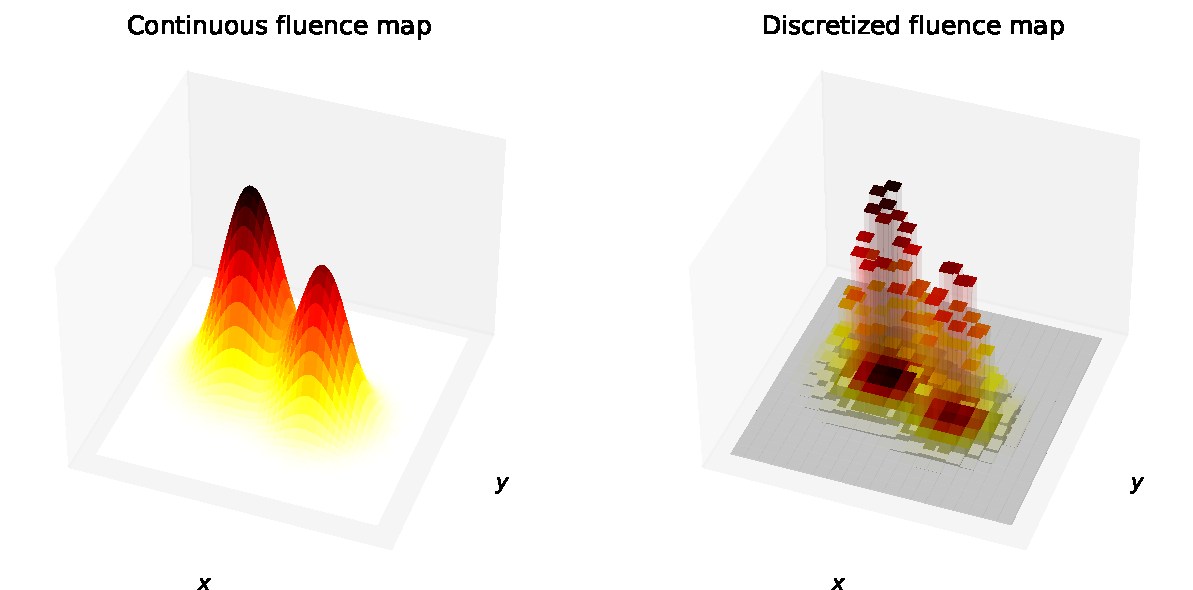
\includegraphics[width=\linewidth]{fluence_discretization_plot3D.pdf}
%		\caption{3D visualization.}
%		\label{fig:fluence_bixel_3D}
%	\end{subfigure}
%	\caption{Example of a fluence discretized to $20 \times 20$ bixels.}
%	\label{fig:fluence_bixel}
%\end{figure}

\begin{figure}
	\centering
	2D visualization
	\\
	\begin{subfigure}[c]{0.45\textwidth}
		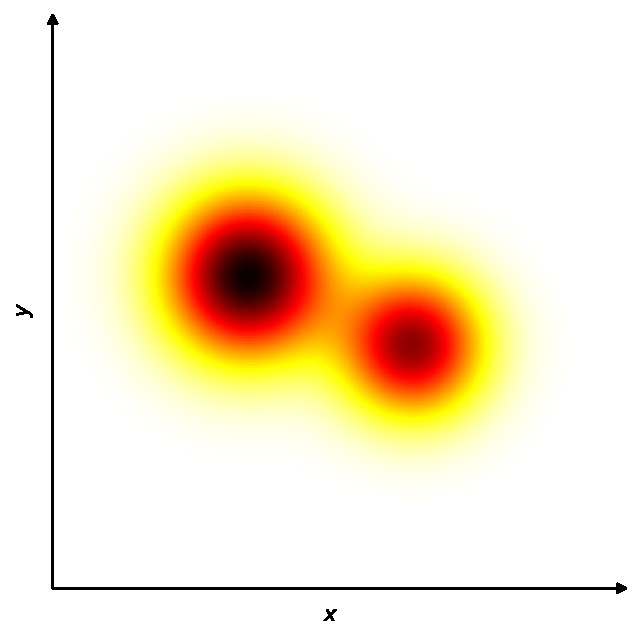
\includegraphics[width=\linewidth]{fluence_continuous_2D.pdf}
		\caption{Continuous fluence (2D plot).}
		\label{fig:fluence_bixel_2D_continuous}
	\end{subfigure}
	\begin{subfigure}[c]{0.45\textwidth}
		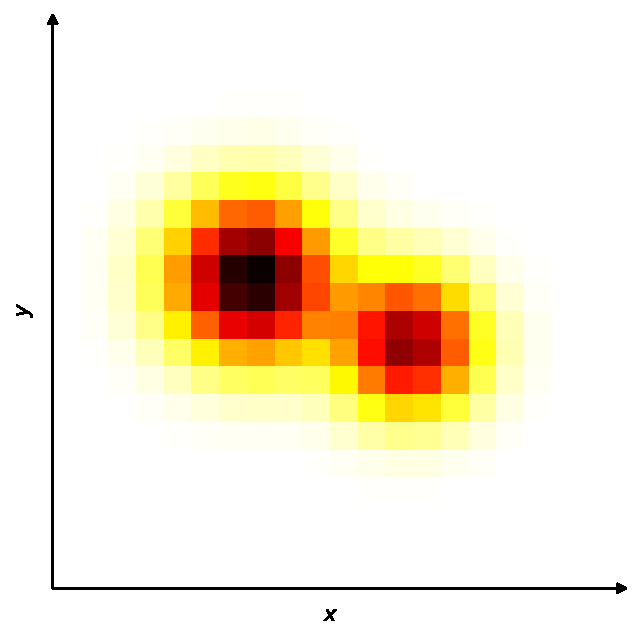
\includegraphics[width=\linewidth]{fluence_discrete_2D.pdf}
		\caption{Discretized fluence (2D plot).}
		\label{fig:fluence_bixel_2D_discrete}
	\end{subfigure}
	\\
	\vspace{5mm}
	3D visualization
	\\
	\begin{subfigure}[c]{0.45\textwidth}
		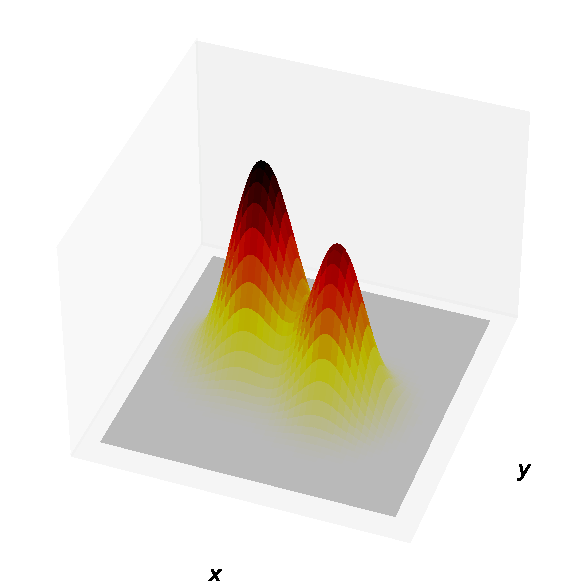
\includegraphics[width=\linewidth]{fluence_continuous_3D.pdf}
		\caption{Continuous fluence (3D plot).}
		\label{fig:fluence_bixel_3D_continuous}
	\end{subfigure}
	\begin{subfigure}[c]{0.45\textwidth}
		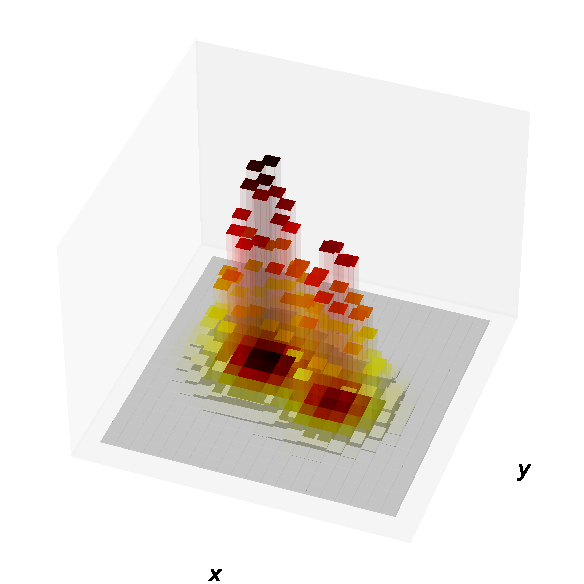
\includegraphics[width=\linewidth]{fluence_discrete_3D.pdf}
		\caption{Discretized fluence (3D plot).}
		\label{fig:fluence_bixel_3D_discrete}
	\end{subfigure}
	\caption{Example of a fluence discretized to $20 \times 20$ bixels.}
	\label{fig:fluence_bixel}
\end{figure}

Fluence maps are broken down into discrete elements called "bixels" (\textbf{be}am \textbf{el}ements).
Bixels represent small and independent beams of radiation (see a visualization figure \ref{fig:fluence_bixel}).

The width of each bixel is constrained by the width of the multi-leaf collimator leaves.
Modern multi-leaf collimator systems typically have a leaf width of 0.5 cm.

The height of a bixel can be selected arbitrarily, as the leaf can move continuously.
Nevertheless, square bixels (akin to image pixels) are commonly used and will be employed throughout this manuscript.

It is essential to know that since negative energy rays are physically infeasible, we need to ensure that each bixel value is non-negative.
Bixels whose beams do not affect the planning target volume are typically excluded from calculations to improve computational efficiency.
Activating these bixels could only degrade dose quality by increasing the dose to organs at risk without benefiting the dose distribution within the planning target volume.

\subsection[Voxels]{Human Body Discretization: Voxels}
The human body of the patient is also divided into discrete elements, as it is a three-dimensional object; the elements are "voxels" (\textbf{vo}lume \textbf{el}ements).
Each voxel represents a small portion of tissue within the patient's body, and will determine the granularity of the dose computed.

The maximum resolution of the voxel grid is defined by the planning image, which is typically a CT scan.
It is common practice to resample the planning image to reduce computational demands.
In this manuscript, where new techniques are explored, we have opted to resample the voxel grid to a resolution of 5 mm, ensuring a balance between computational efficiency and accuracy.

Additionally, to further optimize the computational process, only voxels corresponding to the planning target volume (PTV) and organs at risk (OARs) are retained for calculations.
This selective approach reduces unnecessary computation.

\subsection[DI-Matrix]{Dose-Influence Matrix}
The Dose-Influence Matrix (or DI-Matrix) links the discretized fluence map (the bixels values) and the discretized dose distribution within the patient (the dose on each voxel).
This matrix defines how the radiation from each individual bixel influences the dose delivered to every voxel in the patient's body.

We start by converting the 2D fluence map, composed of individual bixel values, into a column vector $b$.
Similarly, we represent dose distribution in the patient's 3D space as a vector $\mathbf{d}$, where each entry corresponds to the dose in a specific voxel.
The DI-Matrix $L$ governs the relationship between these vectors $\mathbf{b}$ and $\mathbf{d}$ via the matrix-vector multiplication $\mathbf{d} = L\mathbf{b}$.
This mathematical operation computes the total dose at each voxel by summing the contributions from all active bixels (here, we assume that the effect of bixels is linear).

The DI-Matrix is constructed by simulating the radiation delivered by each individual bixel.
For each bixel, the jaws of the multi-leaf collimator are virtually opened to allow only that specific beamlet to go through.
A radiation transport model calculates the dose deposited in each voxel, considering the beam's spread and attenuation as it travels through the body.
The resulting 3D dose deposition fills one column of the matrix $L$, corresponding to that bixel's influence on all voxels.
Repeating this process for each bixel generates the entire DI-Matrix.

The accuracy of the dose calculation depends on the precision of the DI-Matrix.
Simple models like pencil beam approximations, which assume a linear trajectory with minimal scattering, are considered too coarse.
In contrast, more advanced simulations, such as Monte Carlo methods, provide a detailed and accurate dose calculation, although at a higher computational cost.
In this manuscript, we employ collapsed cone convolution techniques (via TheraPanacea dose engine), which balance efficiency and accuracy.

\section{Naive Optimization Method}
\label{naive_optimization}
A natural starting point in dose optimization is to attempt to directly achieve the delivery of a uniform dose, equal to the prescription, on all voxels within the PTV, and no dose elsewhere.
We can attempt to find the bixels values delivering this dose by solving a least squares problem.
We attempt to find the fluence map $\mathbf{b}$ that minimizes the difference between the actual dose $\mathbf{d}$ and the target dose $\mathbf{d}_{\text{target}}$, which is set to the prescribed dose within the PTV.

Formally, the optimization problem can be stated as:
$$ \min_\mathbf{b} \ \| \mathbf{d}_{\text{target}} - L\mathbf{b} \|^2, \quad \mathbf{b} \geq 0$$

where $\mathbf{d}_{\text{target}}$ is the target dose vector, defined as follows for a prescription of $p$Gy:
$$ \mathbf{d}_{\text{target}} = p \cdot  \mathds{1}_{\text{PTV}} $$

Here, $\mathds{1}_{\text{PTV}}$ is the indicator vector for PTV that is equal to $1$ for voxels within the PTV and $0$ elsewhere.

To solve this problem, we perform a least squares minimization to find the optimal fluence map $\mathbf{b}$, where the matrix-vector multiplication $L\mathbf{b}$ yields the dose distribution $\mathbf{d}$ across the entire patient volume.

However, this method is often inadequate in practice, as it attempts to solve the system based solely on the prescribed dose within the PTV, while neglecting any constraints on doses to the organs at risk (OARs).
Since no constraints are imposed on the OAR doses, this naive optimization can result in high doses to critical structures, leading to unacceptable treatment plans.
As a result, more sophisticated optimization methods that incorporate dose constraints on OARs and account for dose-volume constraints are necessary to achieve clinically viable treatment plans.
% add 3D dose & DVHs of dose obtained using this technique

\section{Constraints and Importance Factors}
In order to obtain clinically acceptable doses, we need to incorporate the clinical aims in the optimization.

\subsection{Constraints Formulation}
Different organs exhibit varying sensitivities to radiation, which influence their dose tolerance limits \cite{Withers1988} \cite{ICRU83}.
Normal tissues are categorized as serial, parallel, or mixed, based on the functional organization of their sub-units.
This classification determines the appropriate absorbed dose limits for normal tissues.

Serial organs (figure \ref{fig:serial_organ}), such as the spinal cord or esophagus, are characterized by a functional dependence on the integrity of every sub-unit.
Damage to even a tiny region in these tissues can result in the loss of the organ's overall function.
In contrast, parallel organs (figure \ref{fig:parallel_organ}), such as the lung or liver, possess a reserve capacity where damage to a portion of the tissue does not necessarily impair overall function, as long as a critical volume remains intact.

\begin{figure}
	\begin{subfigure}{0.6\textwidth}
		\centering
		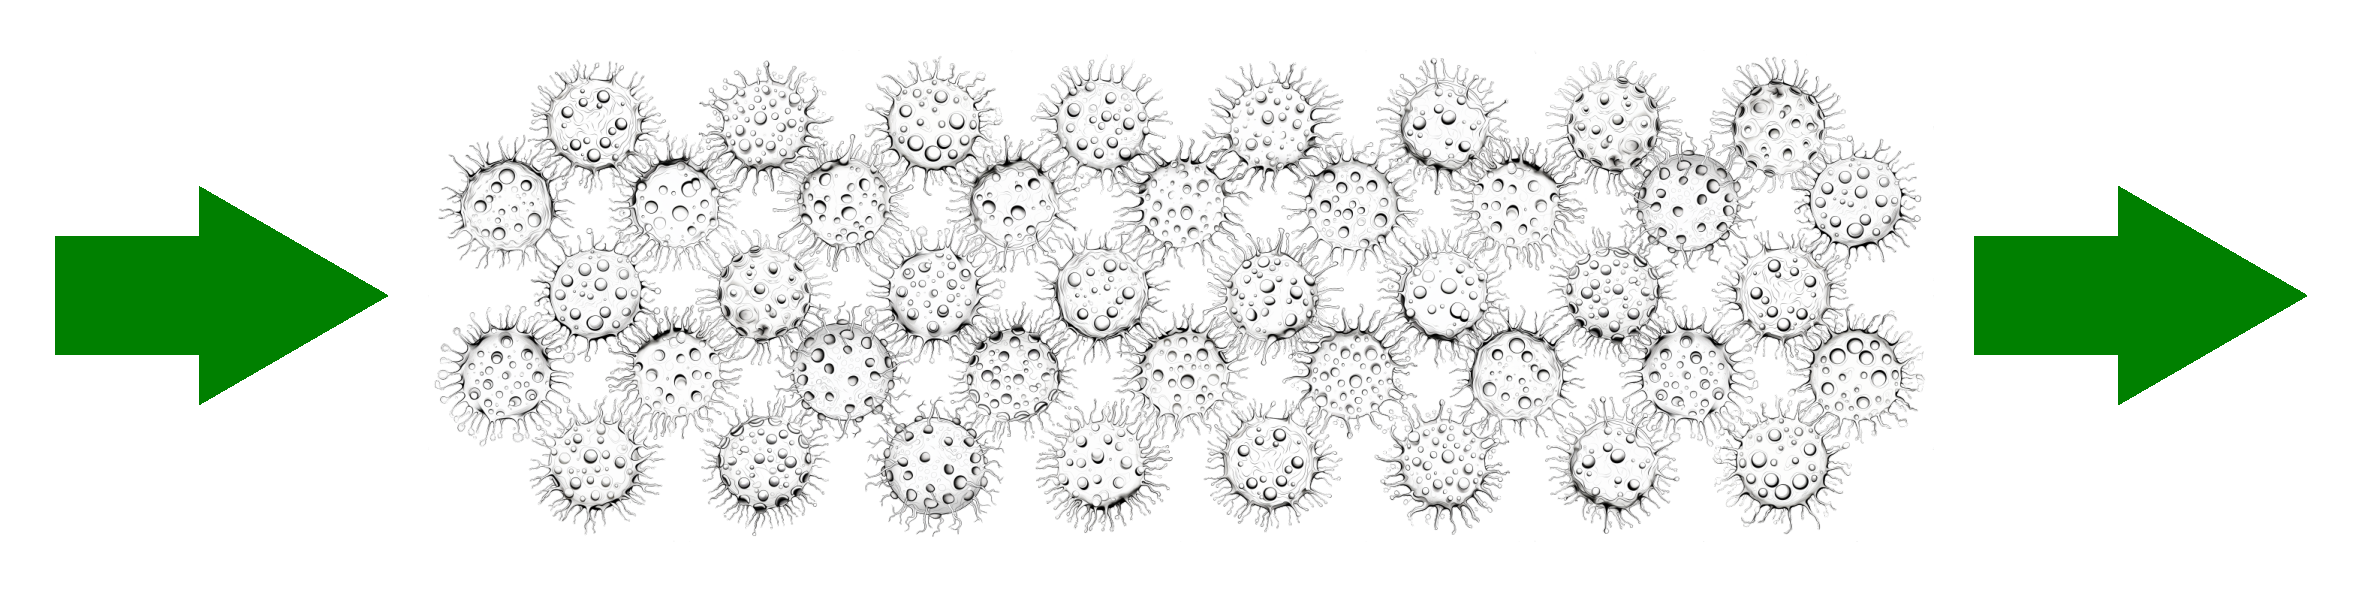
\includegraphics[width=0.9\textwidth]{serial_organ.pdf}
		\vspace{4mm}
		\caption{Organ functioning in a serial-like way.}
		\label{fig:serial_organ}
	\end{subfigure}
	\hfill
	\unskip\ \vrule\
	\hfill
	\begin{subfigure}{0.38\textwidth}
		\centering
		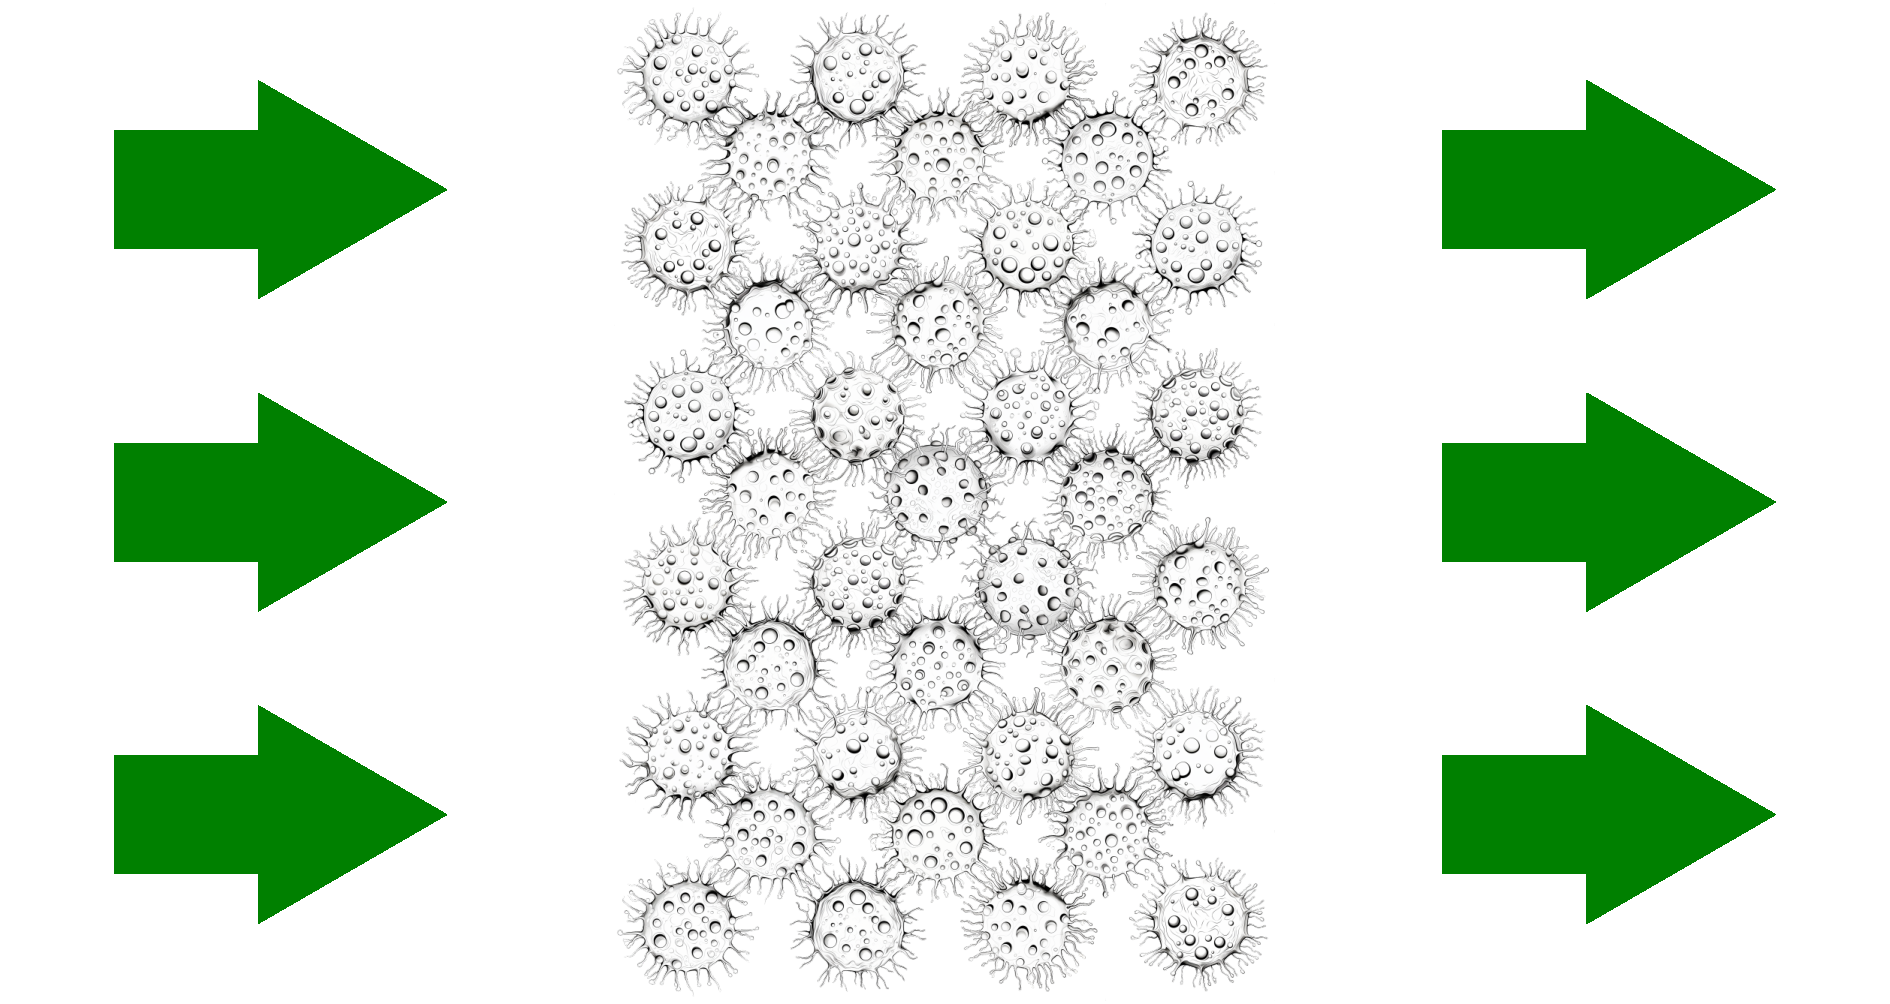
\includegraphics[width=0.9\textwidth]{parallel_organ.pdf}
		\caption{Organ functioning in a parallel-like way.}
		\label{fig:parallel_organ}
	\end{subfigure}
	\caption{Organs functioning types.}
	\label{fig:serial_parallel_organ}	
\end{figure}

We define two DVH value measures, $V_X$ and $D_{X\%}$, for a structure $S$.
For a given dose $d: \R^3 \to \R^+$, $V_X$ is defined as the volume of the three dimensional structure $S \subseteq \R^3$ that receives a dose equal to or higher than $X$, that is:
$$ V_X = \frac{\vol{\left\lbrace p \in S \subset \R^3 \mid d(p) \geq X \right\rbrace}}{\vol{S}}.$$
This formula can be approximated using the discretized dose on voxels $\mathbf{d}$:
$$ V_X \approx \frac{ \#{\left\lbrace v \in S \mid \mathbf{d}_v \geq X \right\rbrace}}{\#\left\{ v \in S \right\}}$$
with $v \in S$ voxels of the structure $S$, $\mathbf{d}_v$ the dose of $\mathbf{d}$ associated with voxel $v$, and $\#$ refers to voxel count.

Similarly, we define $D_{X\%}$ as the minimal dose (in Gy) delivered to the $X\%$ most irradiated region of the structure, that is:
$$D_{X\%} = \min \left\lbrace d(p) \mid p \in S_{X\%} \right\rbrace$$
where $S_{X\%} \subseteq S$ is the $X\%$ most irradiated region of $S$.
Again, it can be approximated using the discretized dose on voxels $\mathbf{d}$:
$$D_{X\%} \approx \min \left\lbrace \mathbf{d}_v \mid v \in S_{X\%} \right\rbrace$$
where $v \in S_{X\%}$ are the $X\%$ most irradiated voxels of $S$.

For parallel-like structures, dose–volume reporting specifying $V_D$ is commonly used, with $D$ adapted to the specific organ.
For instance, \cite{Graham1995} demonstrated a correlation between the incidence and severity of lung pneumonitis and $V_{20 \text{ Gy}}$, the volume of the lung receiving more than 20 Gy.
In parallel-like structures, the median absorbed dose ($D_{50\%}$) provides a valuable measure of the total dose delivered to the organ at risk.

For serial-like organs, it is recommended to report $D_{2\%}$ as the maximum absorbed dose, as $D_{0\%}$ is subject to noise.

Finally, for organs with a mixed parallel-serial structure, it is advised to report $D_{50\%}$, $D_{2\%}$, and $V_D$, with $D$ selected based on the threshold beyond which there is a significant risk of serious complications.

\begin{figure}
	\begin{subfigure}[b]{0.48\textwidth}
		\caption{Irradiation of organs at risk with one heat point.}
		\label{fig:organ_radiation_point}
		\centering
		\vspace{3mm}
		\hspace{1.2cm}
		Treatment Dose
		\\
		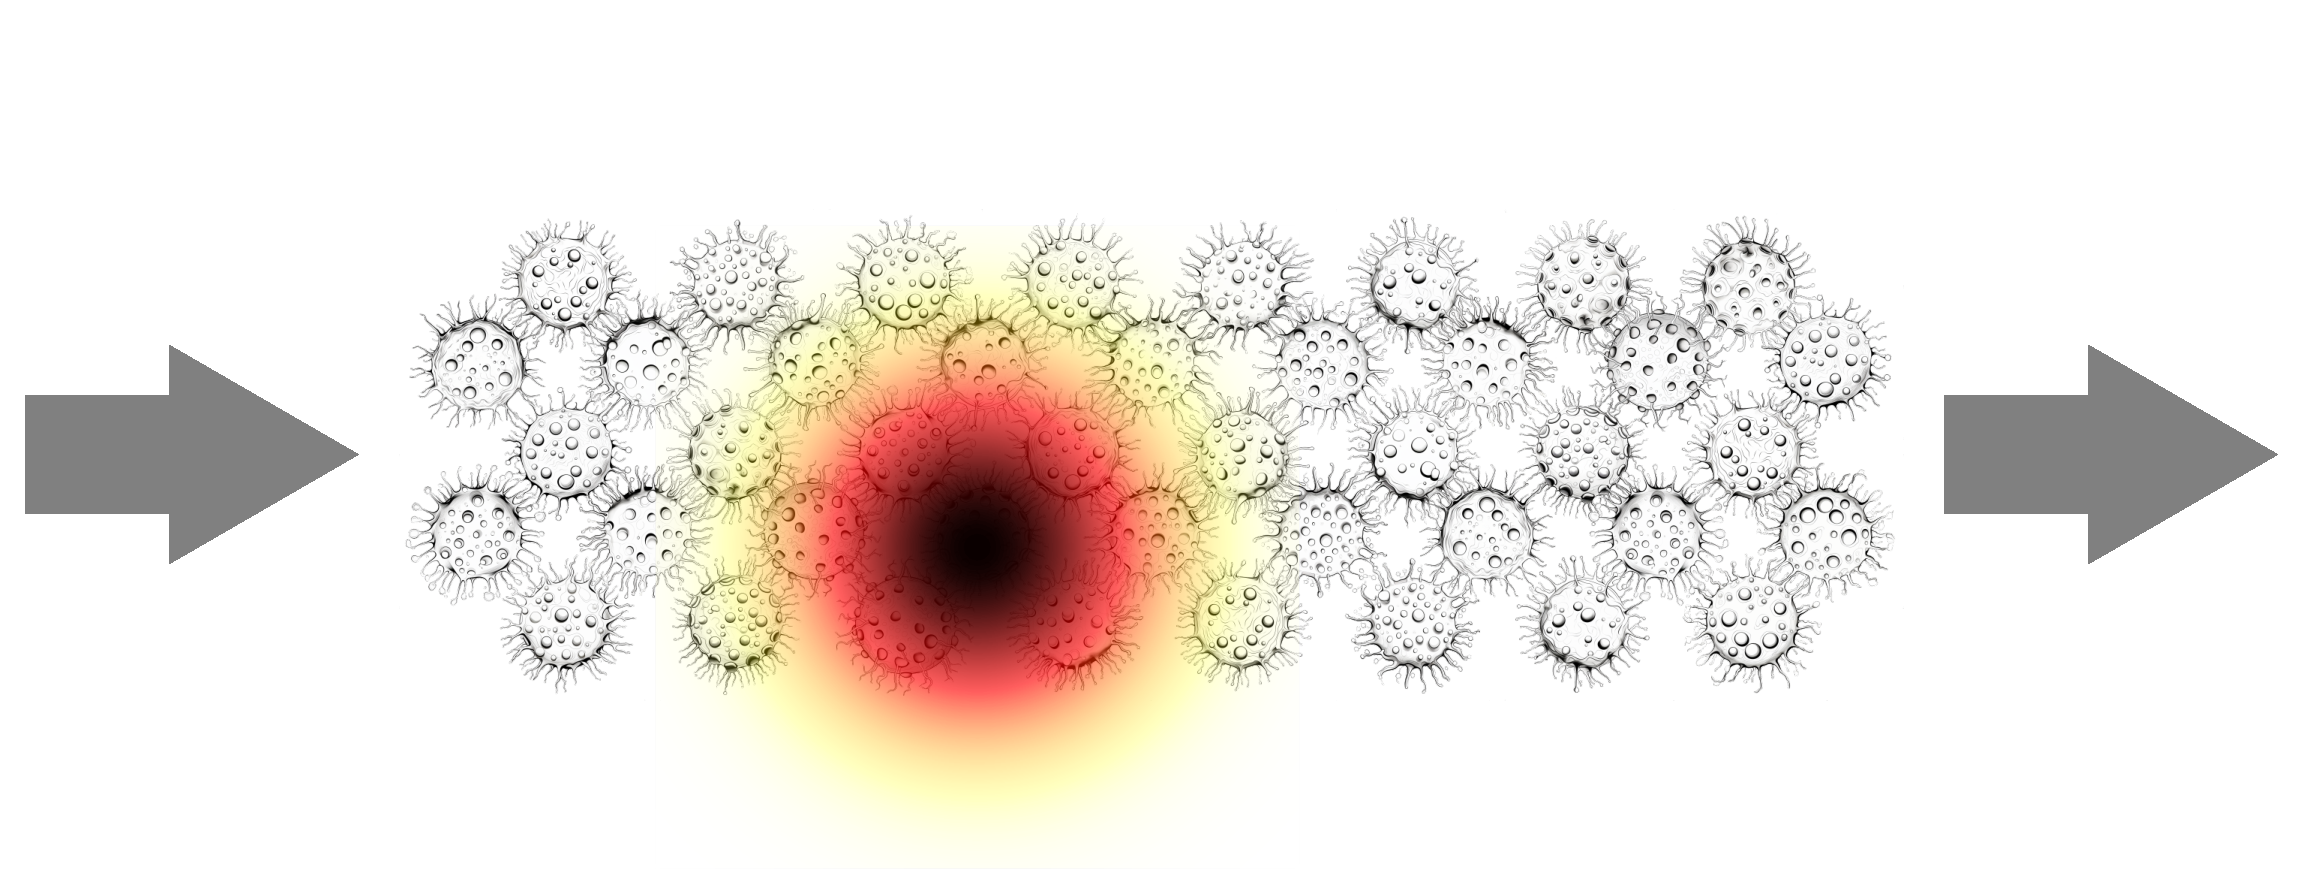
\includegraphics[width=0.55\textwidth]{serial_heat_point.pdf}
		\vbar
		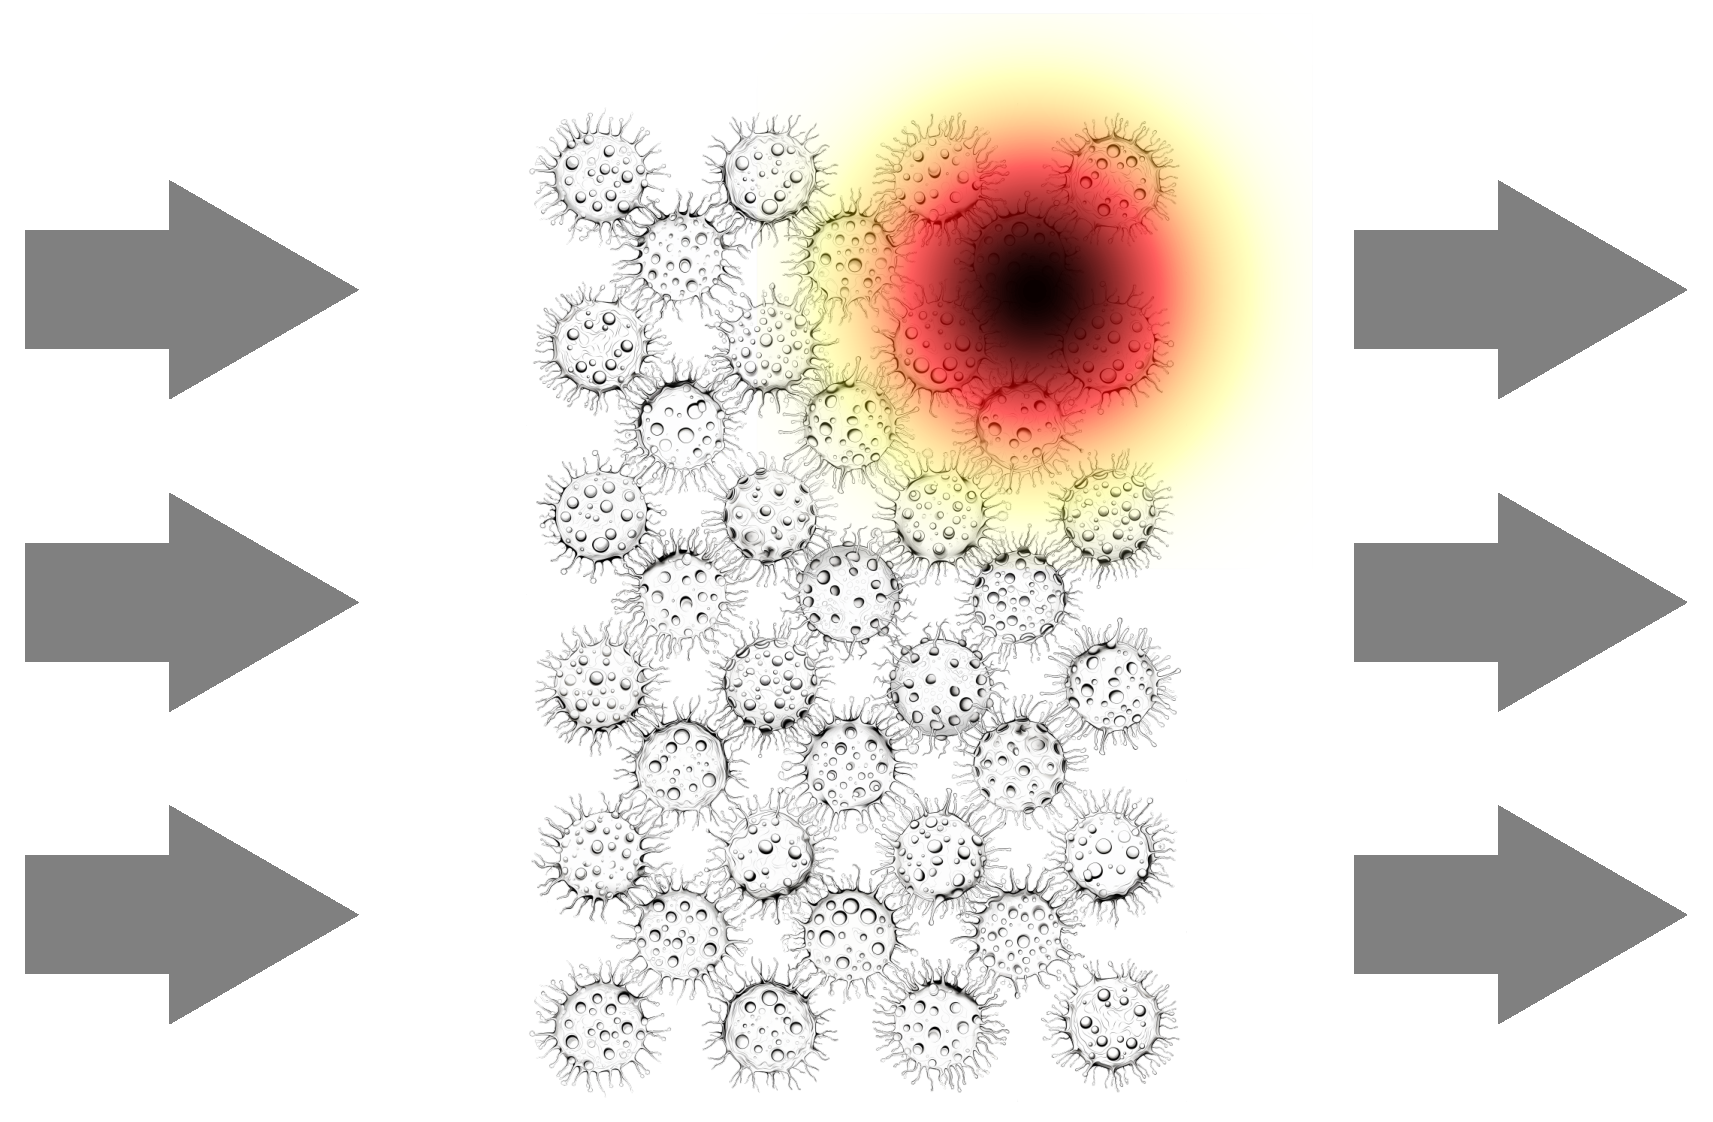
\includegraphics[width=0.35\textwidth]{parallel_heat_point.pdf}
		\\
		\hspace{1.1cm}
		Post Treatment
		\\
		\noindent
		\begin{subfigure}[b]{0.55\textwidth}
			\addtocounter{subfigure}{-1}
			\renewcommand\thesubfigure{\alph{subfigure}1}
			\centering
			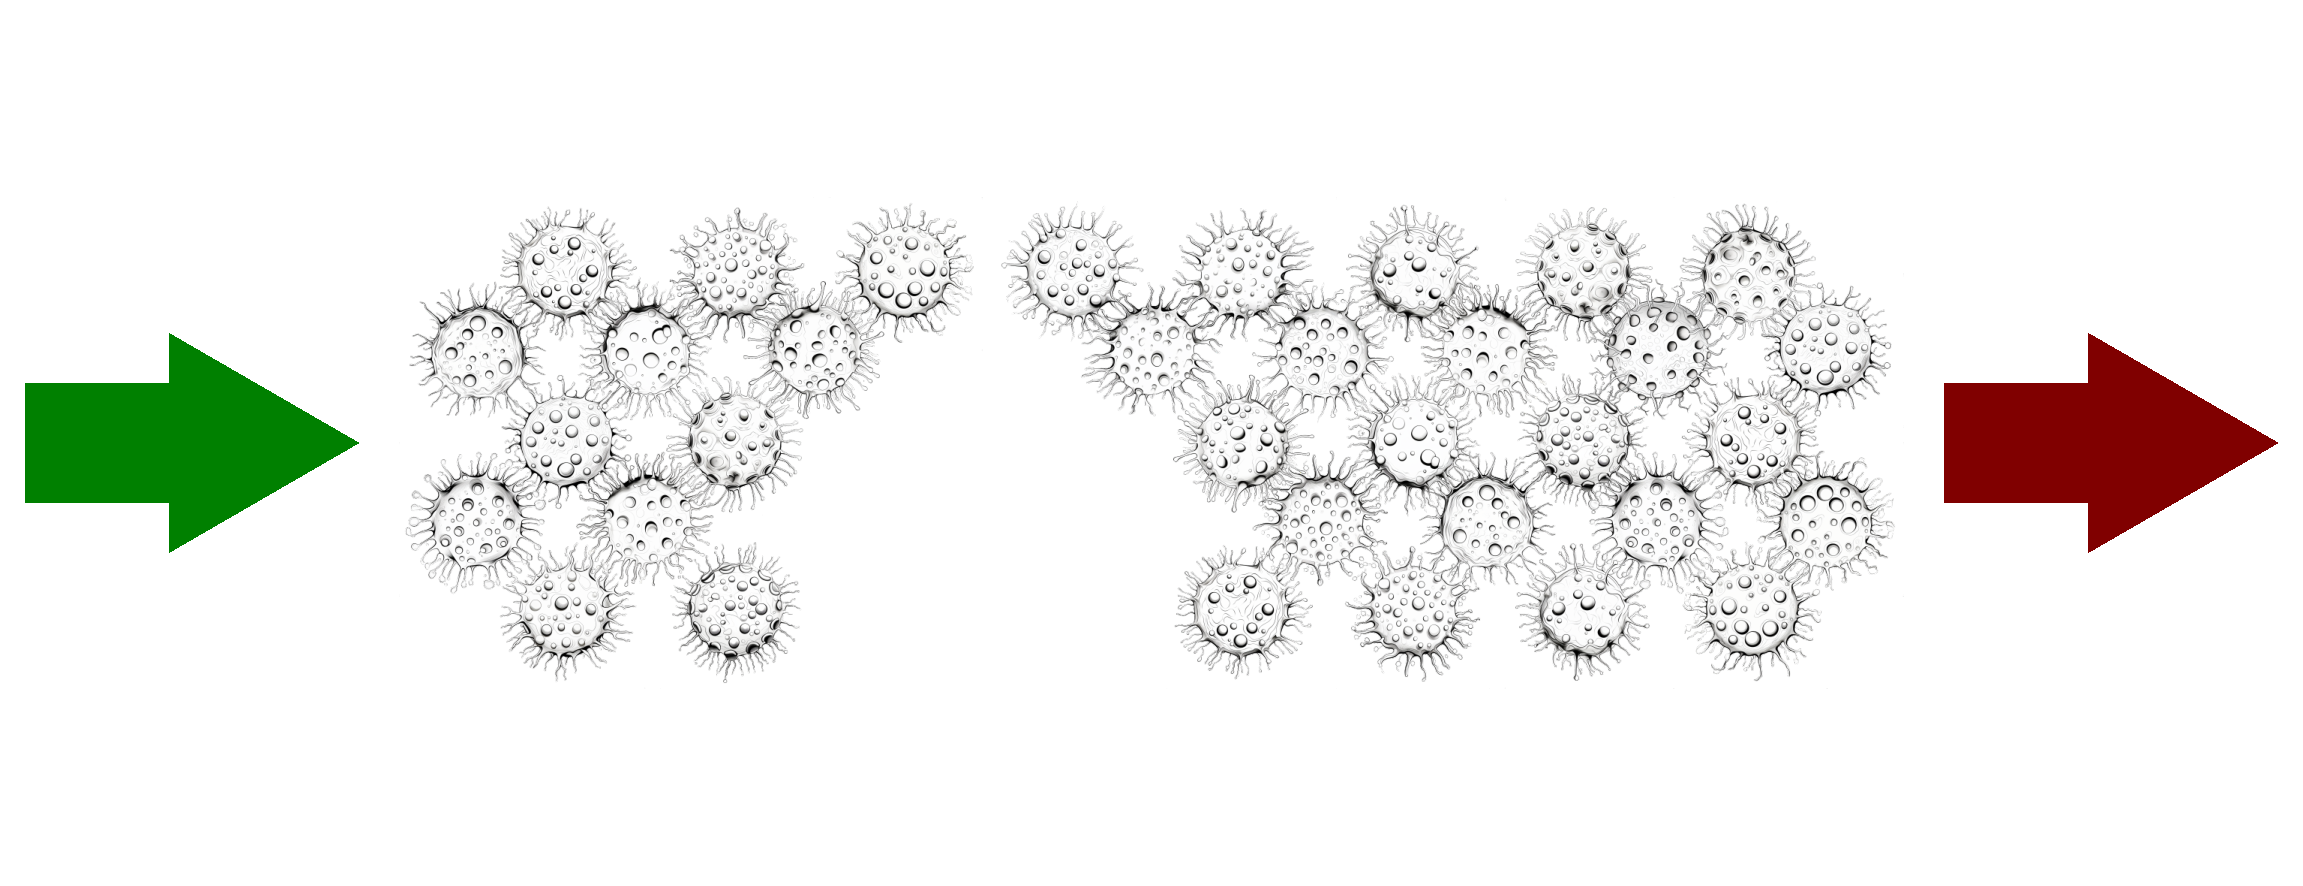
\includegraphics[width=\textwidth]{serial_heat_point_post.pdf}
			\vspace{0.5mm}
			\caption{Serial organ dies.}
		\end{subfigure}
		\vbar
		\begin{subfigure}[b]{0.35\textwidth}
			\addtocounter{subfigure}{-1}
			\renewcommand\thesubfigure{\alph{subfigure}2}
			\centering
			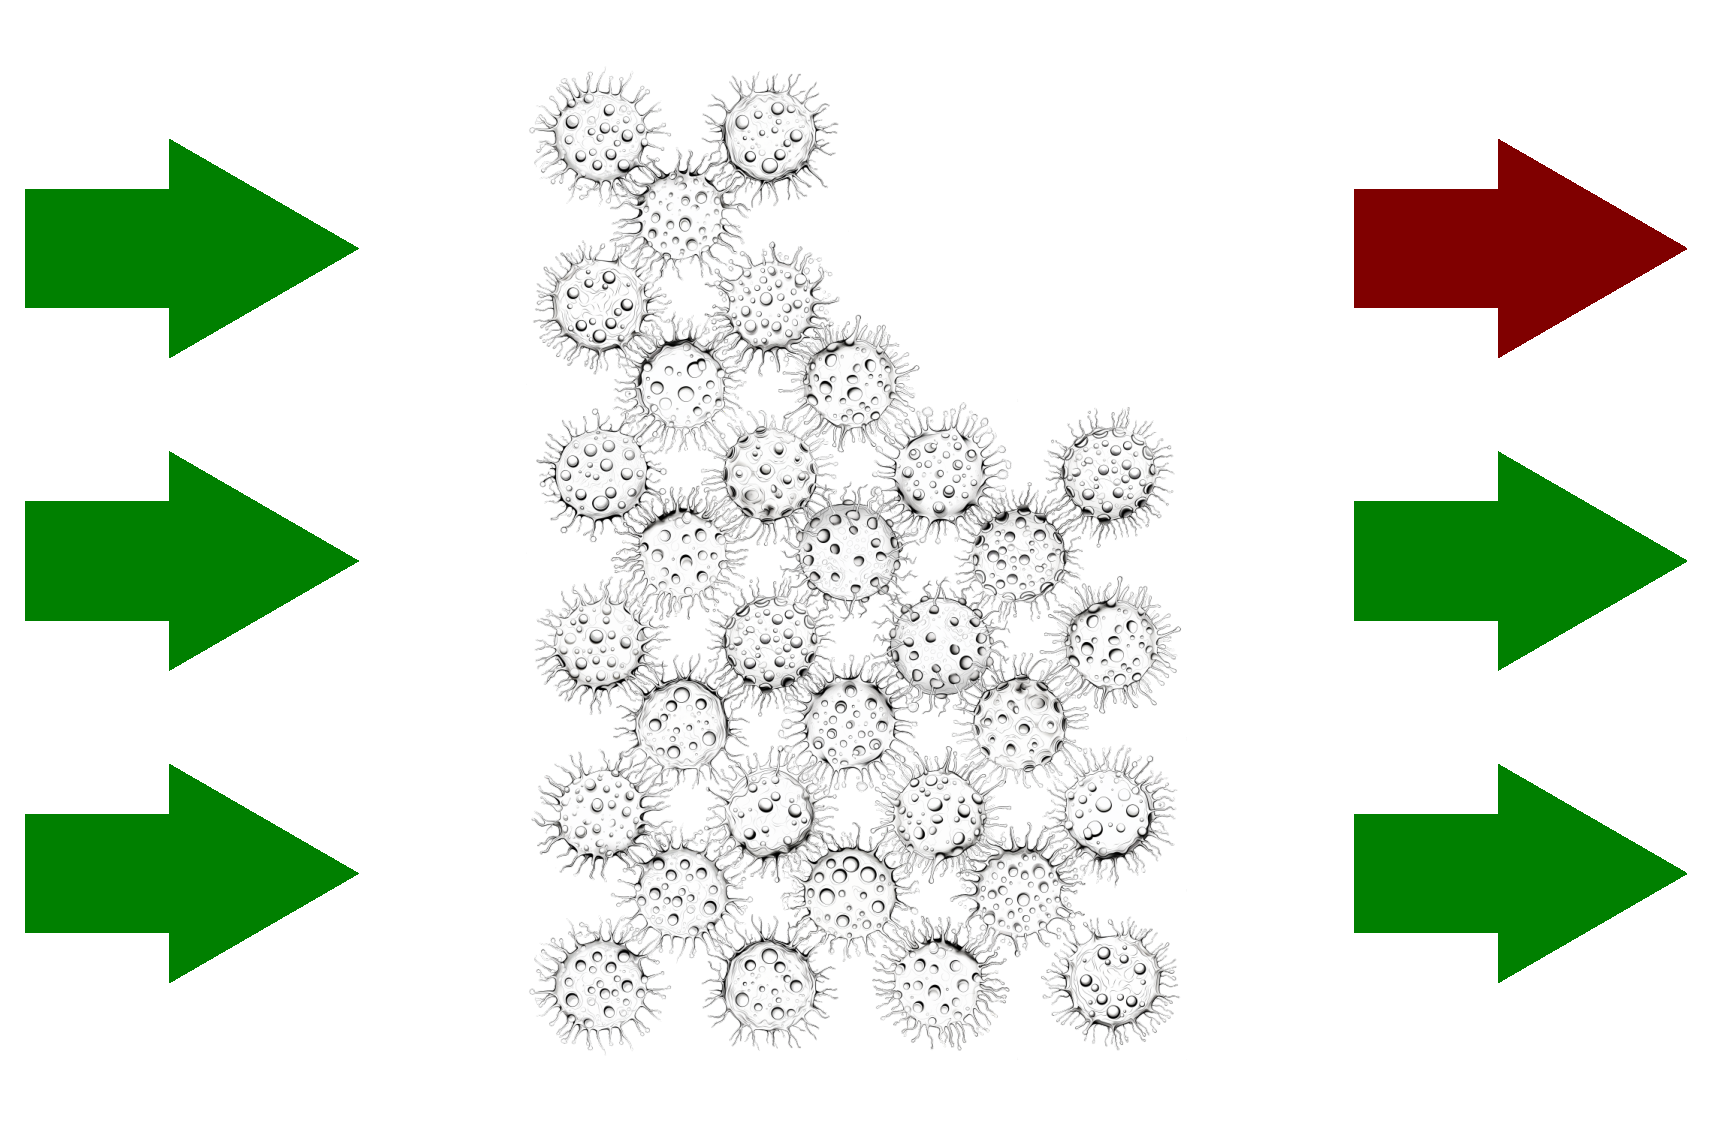
\includegraphics[width=\textwidth]{parallel_heat_point_post.pdf}
			\caption{Parallel organ survives.}
		\end{subfigure}	
	\end{subfigure}
	\vbar
	\begin{subfigure}[b]{0.48\textwidth}
		\caption{Irradiation of organs at risk with spread heat dose.}
		\label{fig:organ_radiation_square}
		\centering
		\vspace{3mm}
		\hspace{1.2cm}
		Treatment Dose
		\\
		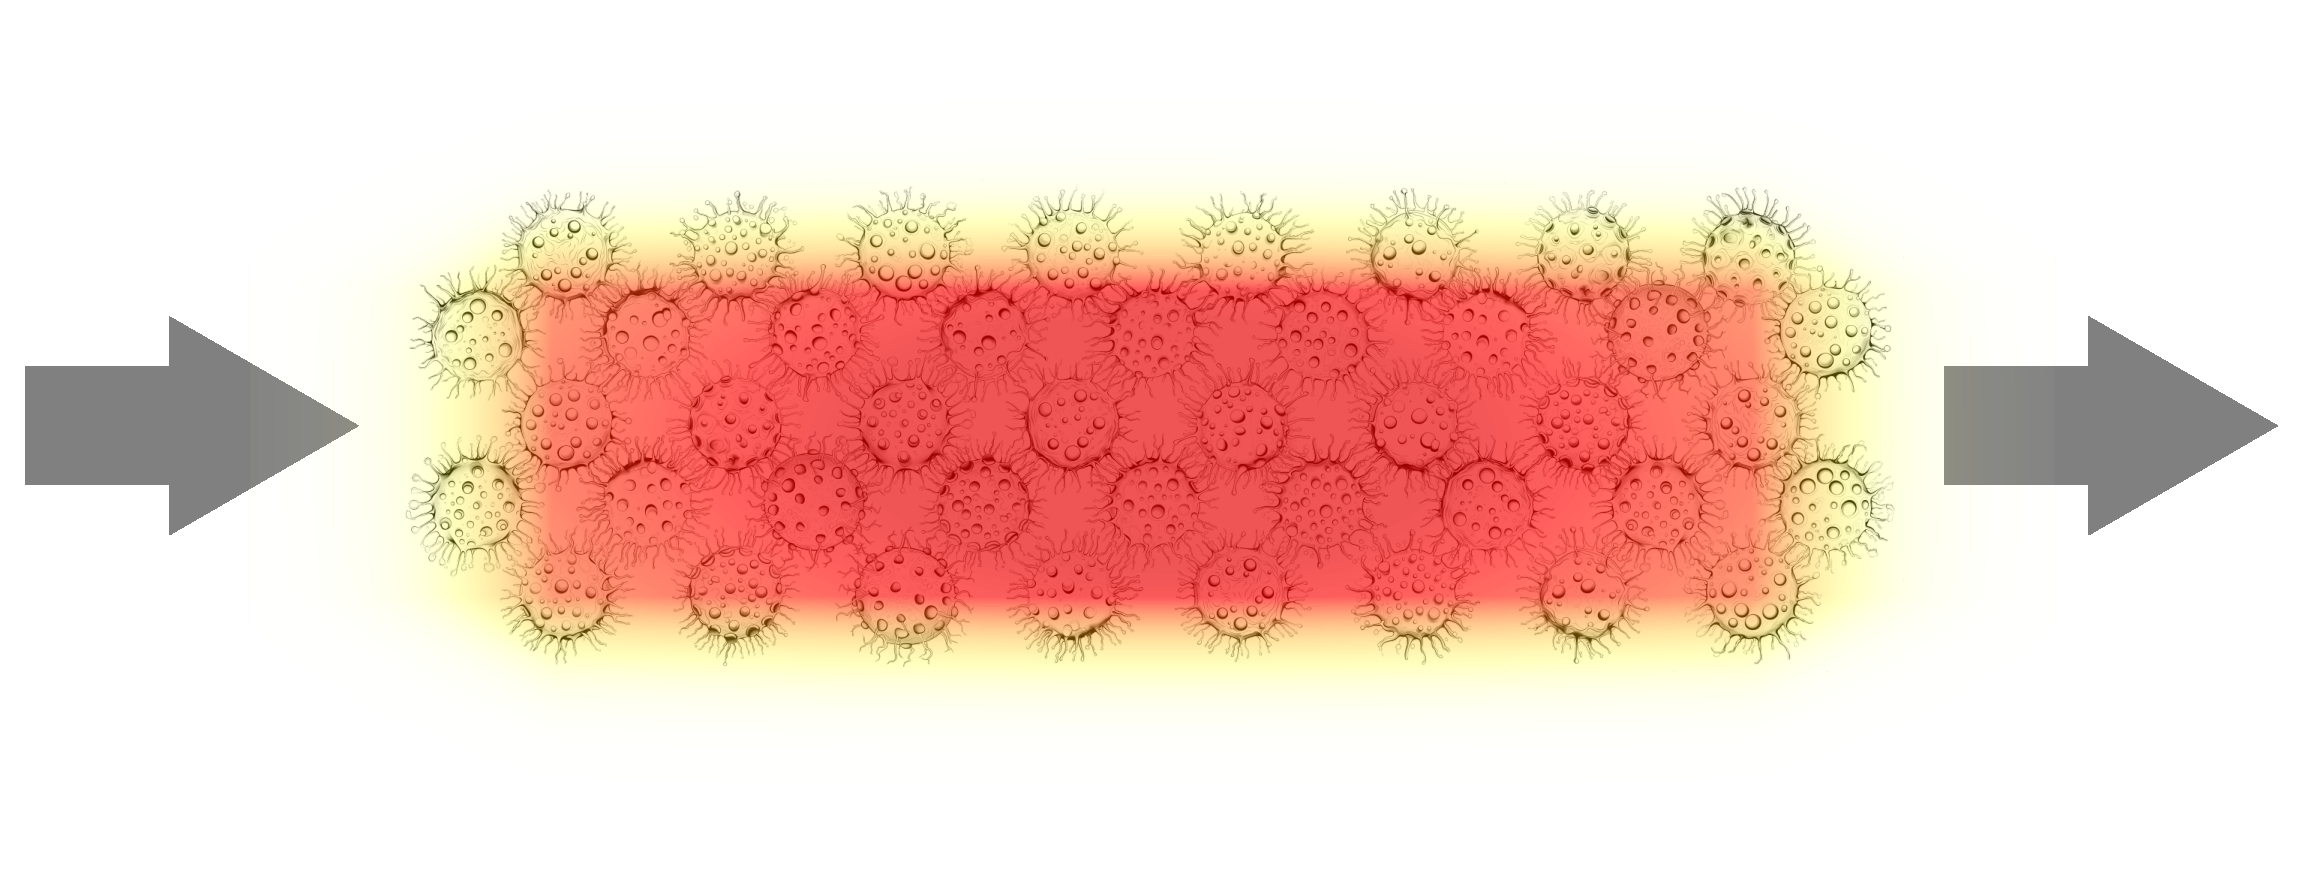
\includegraphics[width=0.55\textwidth]{serial_heat_square.pdf}
		\vbar
		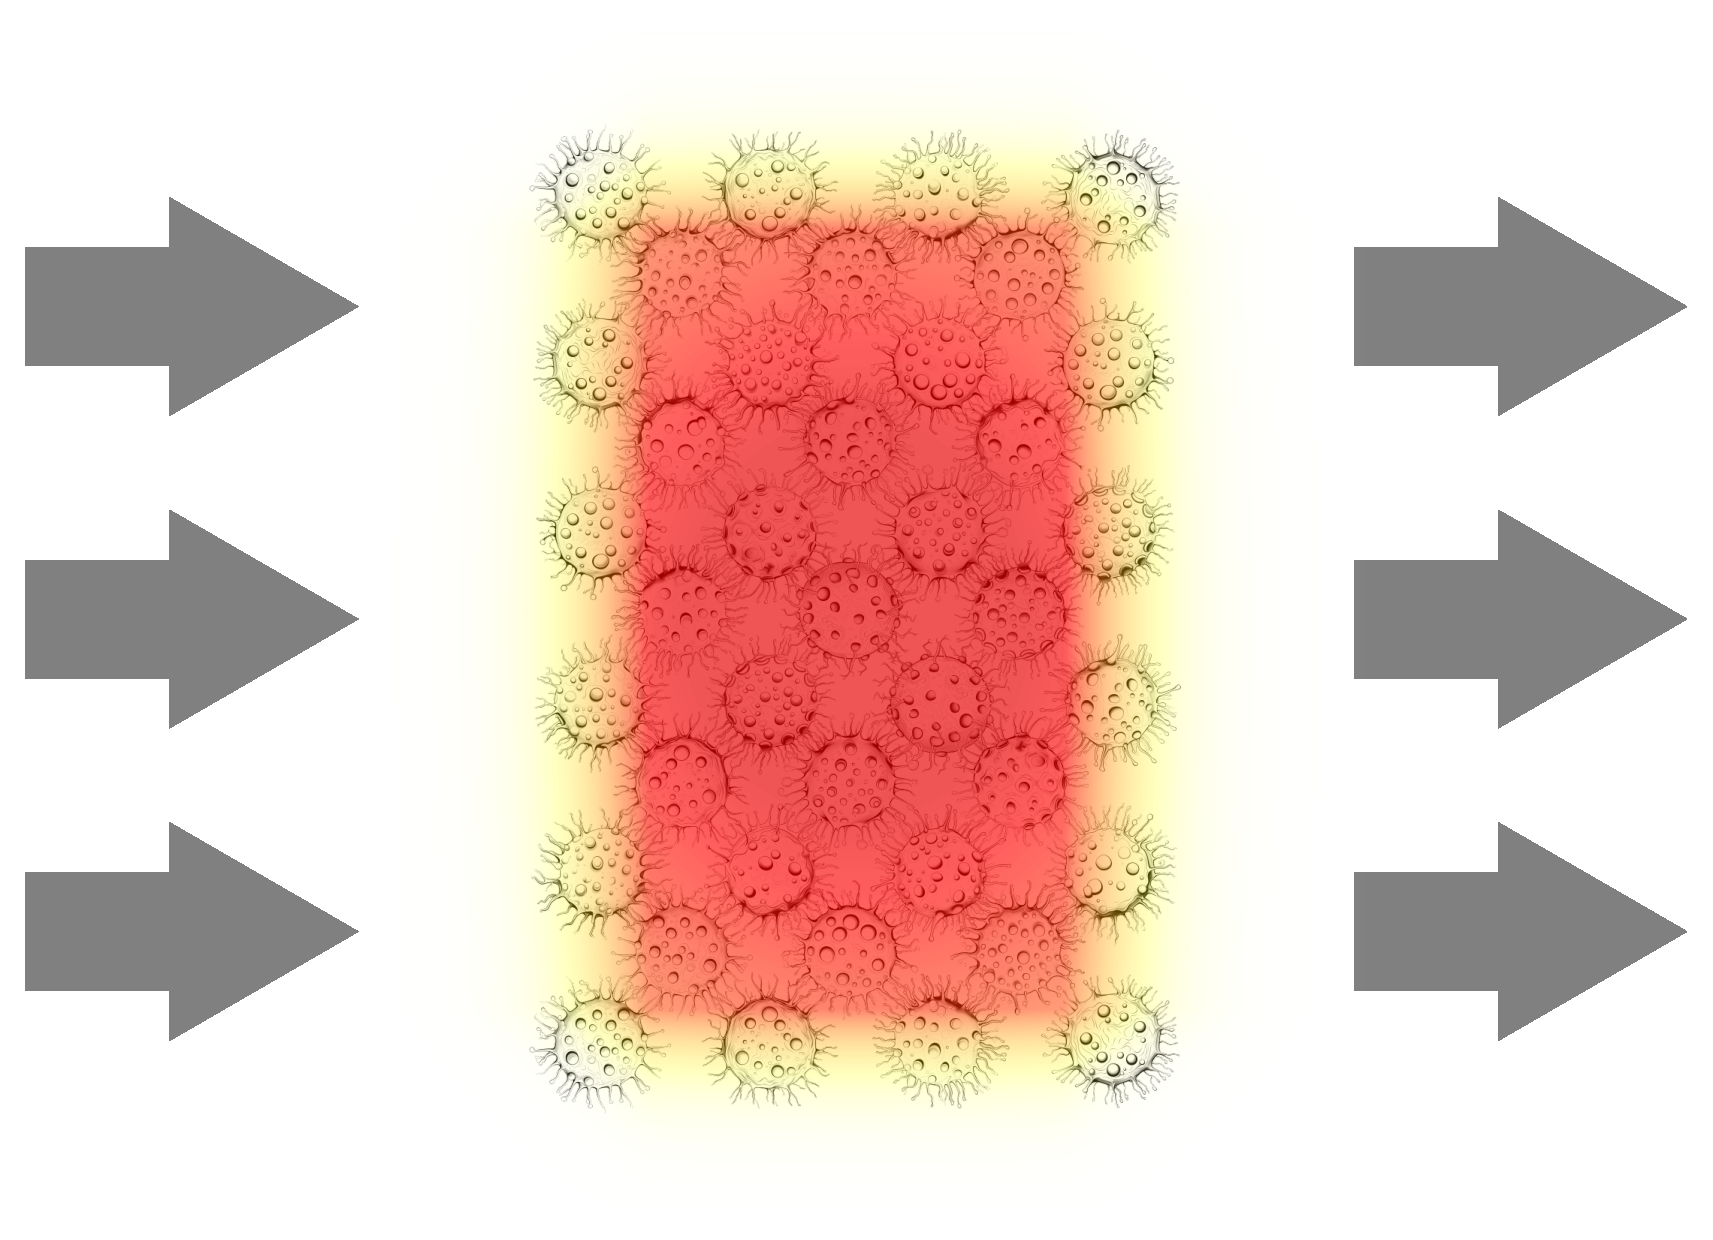
\includegraphics[width=0.35\textwidth]{parallel_heat_square.pdf}
		\\
		\hspace{1.1cm}
		Post Treatment
		\\
		\noindent
		\begin{subfigure}[b]{0.55\textwidth}
			\addtocounter{subfigure}{-1}
			\renewcommand\thesubfigure{\alph{subfigure}1}
			\centering
			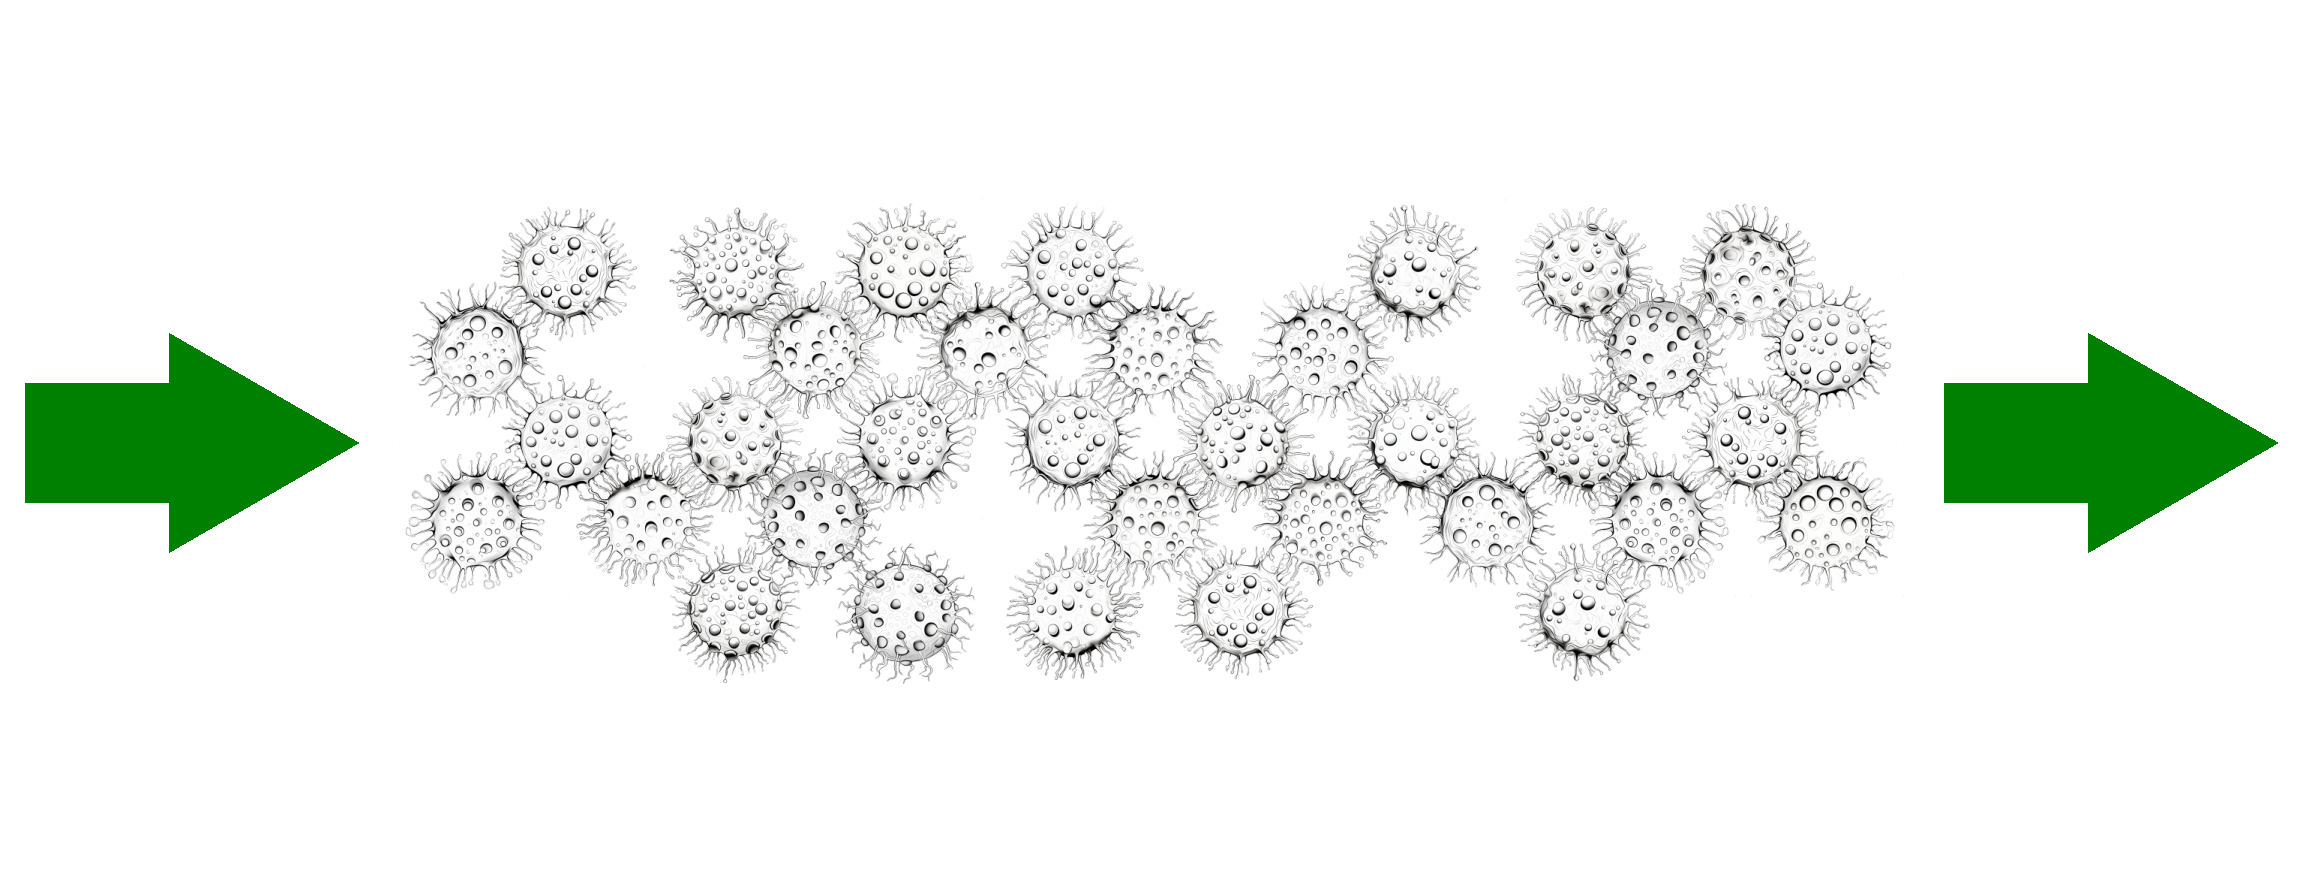
\includegraphics[width=\textwidth]{serial_heat_square_post.pdf}
			\vspace{0.5mm}
			\caption{Serial organ survives.}
		\end{subfigure}
		\vbar
		\begin{subfigure}[b]{0.35\textwidth}
			\addtocounter{subfigure}{-1}
			\renewcommand\thesubfigure{\alph{subfigure}2}
			\centering
			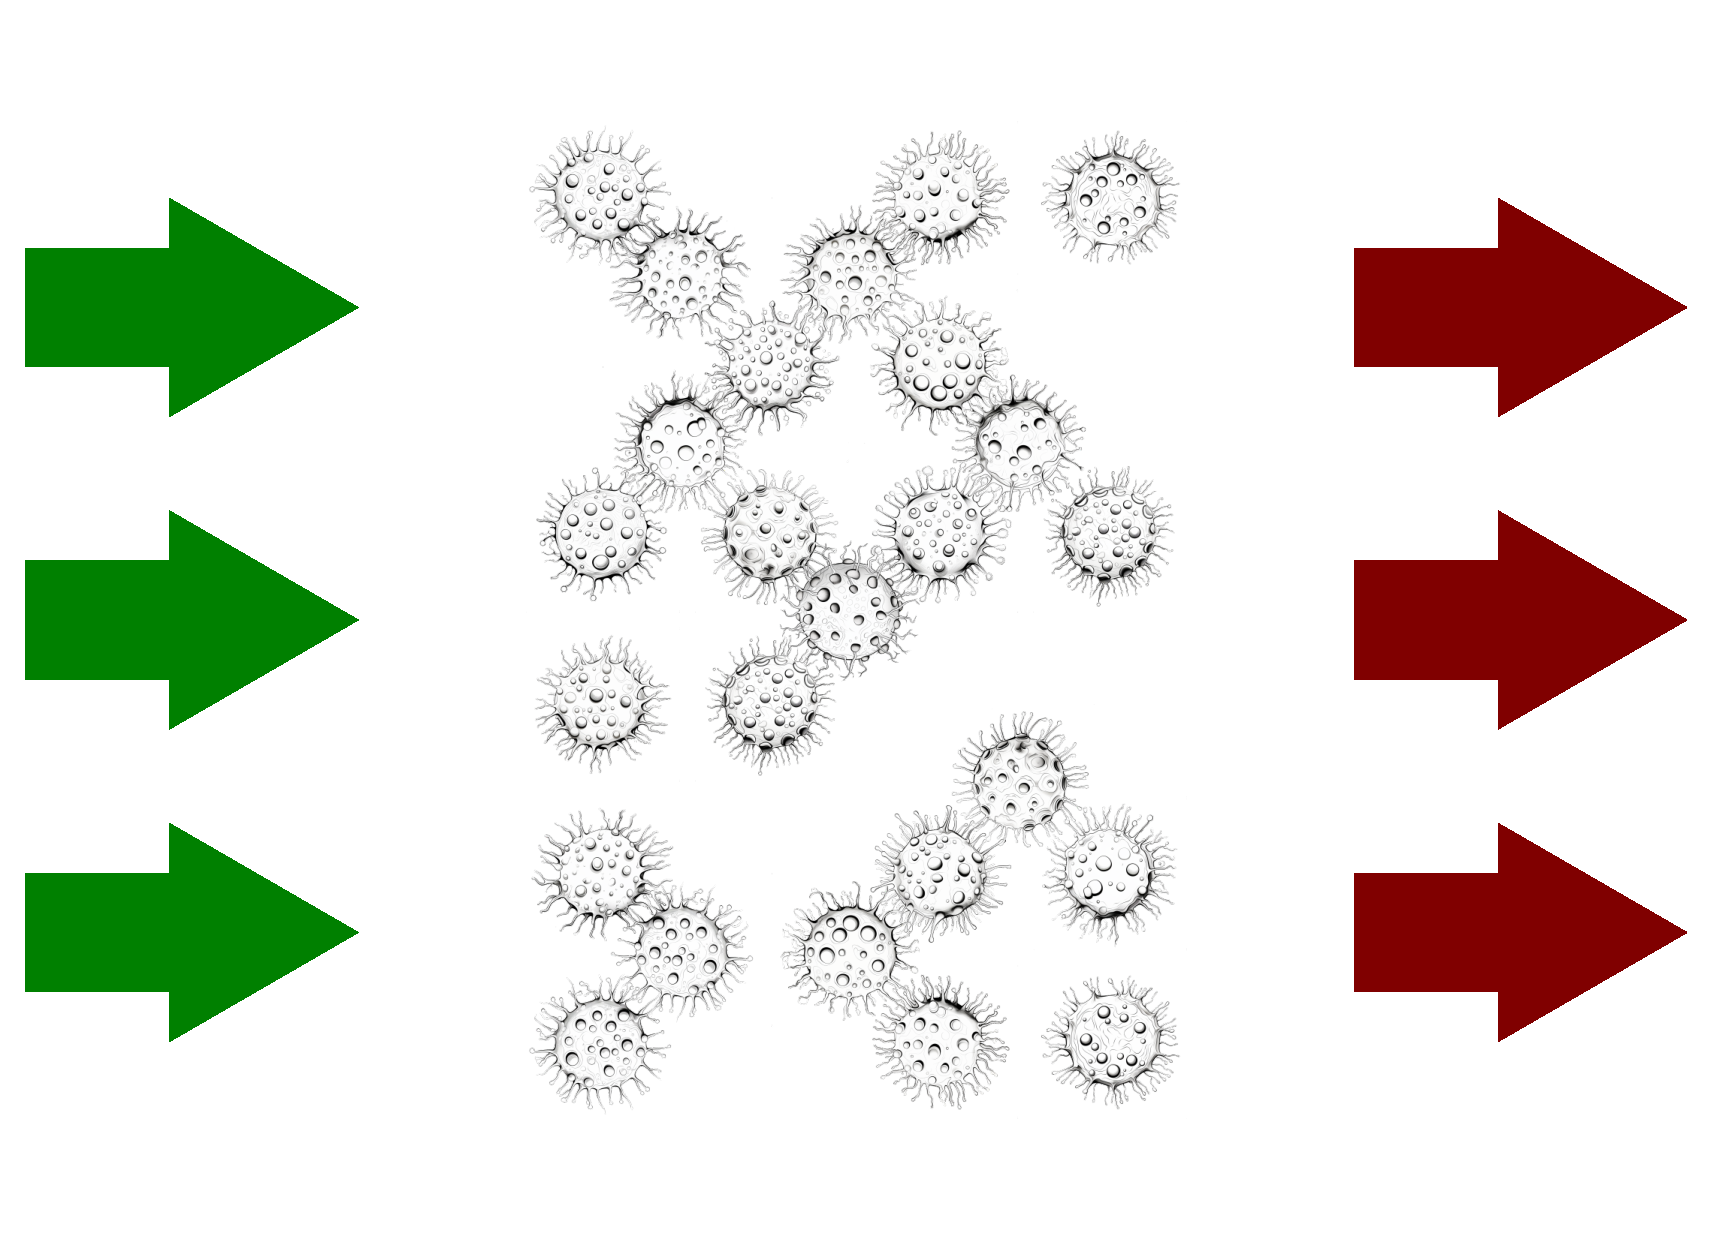
\includegraphics[width=\textwidth]{parallel_heat_square_post.pdf}
			\caption{Parallel organ dies.}
		\end{subfigure}	
	\end{subfigure}
	\addtocounter{subfigure}{-1}
	\caption{Irradiation type survival of organs serial-like and parallel-like.}
	\label{fig:serial_parallel_organ_radiation}
\end{figure}

\subsection{Optimization Problem}
After the doctors have formulated maximal dose constraints for each OARs, and PTV coverage constraints $\mathcal{C}$, we can formulate the mathematical optimization problem.

Constraints $c \in \mathcal{C}$ are formulated as $c = \left( S, D, V, \pm \right)$ where $D$ is in Grey, $V$ is a \%, and $\pm$ means the constraint is maximal/minimal.
\\
\textit{\textbf{E.g.:}} $c_{PTV+} = \left( \text{PTV}, \ 76\,Gy, \ 95\,\%, \ + \right)$ means that for the PTV structure, we need $D_{95\%} \geq 76\,\textit{Gy}$ (or, equivalently, $V_{76\textit{Gy}} \geq 95 \%$); this is a very typical constraint \cite{Zhao2016}.
\\
\textit{\textbf{E.g. (bis):}} $c_{\text{organ}} = \left( \text{organ}, \ 25\, Gy, \ 20\,\%, \ - \right)$ means that for the 'organ' structure, we need $D_{20\%} \leq 25\,\textit{Gy}$ (or, equivalently, $V_{25\textit{Gy}} \leq 25 \%$).
This constraint example is illustrated in figure \ref{fig:constraint_plot_unmet}, \ref{fig:constraint_plot_met}, \ref{fig:constraint_plot_min}.

\begin{figure}
	\centering
	\begin{subfigure}{0.32\textwidth}
		\centering
		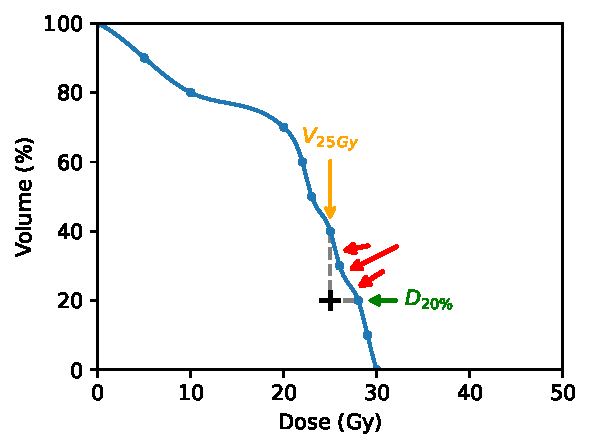
\includegraphics[width=0.9\textwidth]{constraint_plot.pdf}
		\caption{Maximal dose constraint not met.}
		\label{fig:constraint_plot_unmet}
	\end{subfigure}
	\begin{subfigure}{0.32\textwidth}
		\centering
		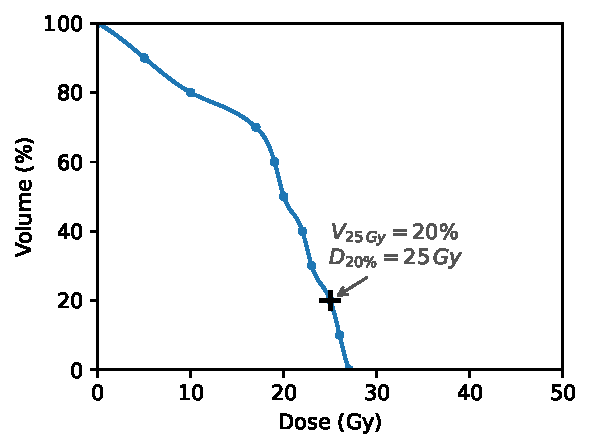
\includegraphics[width=0.9\textwidth]{constraint_plot_met.pdf}
		\caption{Maximal dose constraint met.}
		\label{fig:constraint_plot_met}
	\end{subfigure}
	\begin{subfigure}{0.32\textwidth}
		\centering
		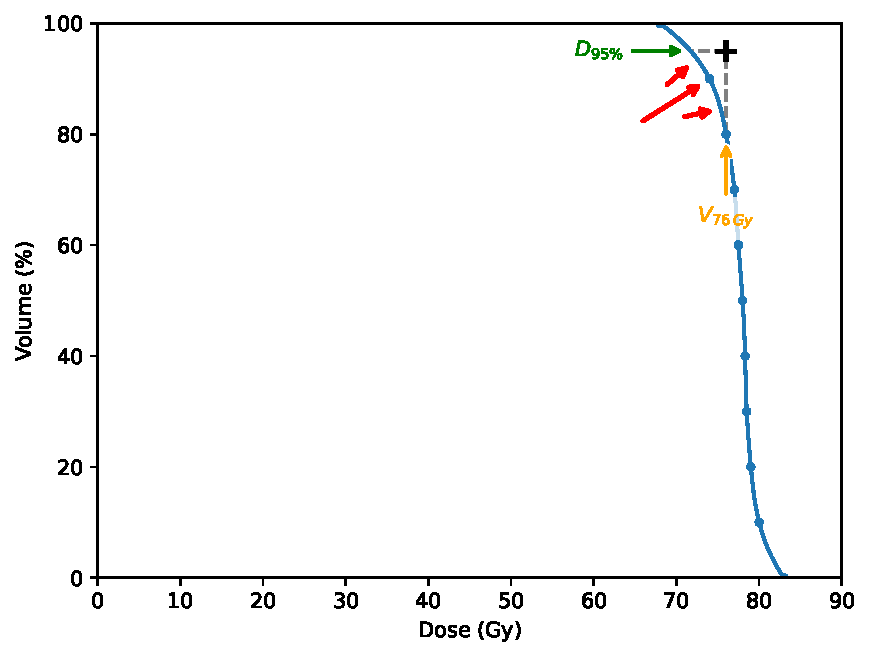
\includegraphics[width=0.9\textwidth]{constraint_plot_min.pdf}
		\caption{Minimal dose constraint unmet.}
		\label{fig:constraint_plot_min}
	\end{subfigure}
	\caption*{
		Figures \ref{fig:constraint_plot_unmet}, \ref{fig:constraint_plot_met}:
		Typical DVH of an OAR, with visualization of the maximal dose constraint $D_{20\%} \leq 25\,\text{Gy}$ (or $V_{25\text{Gy}} \leq 20\,\%$).\\
		Figure \ref{fig:constraint_plot_min}:
		Typical DVH of a PTV, with visualization of the minimal dose constraint $D_{95\%} \geq 76\,\text{Gy}$ (or $V_{76\text{Gy}} \geq 95\,\%$).\\
		Note that dose-volume objectives then turn to points on dose-volume histograms.
		The relevant DVH curve must stay above (in the case of a minimal dose constraint), or under (in the case of a maximal dose constraint) this point to pass the constraint.
	}
	\label{fig:constraint_plot}
\end{figure}

We only calculate a voxel-discretized version $\mathbf{d}$ of the dose $d: \R^3 \to \R^+$, using a bixel-discretized version $\mathbf{b}$ of the fluence maps $f^\theta: \R^2 \to \R^+$ for each selected angle $\theta$.
Hence, we formulate the optimization problem on the discretized information.

\paragraph{Ideal Case}
In the ideal case, it is possible to meet all constraints, and we try to minimize further the dose $\mathbf{d}$ on the OARs.
Mathematically, we find the values for $\mathbf{b}$ giving dose $\mathbf{d} = L\mathbf{d}$ such that all DVH constraints $\mathcal{C}$ are satisfied, and $\sum_{v \in \text{OARs}} \mathbf{d}_v^2 \ $ is minimum (where $\mathbf{d}_v$ is the dose on voxel $v$, and $v \in \text{OARs}$ are the voxels $v$ belonging to an OAR):
$$
\min_{\mathbf{b}} \sum_{v \in \text{OARs}} \ \mathbf{d}_v^2
\quad \text{ with }
\mathbf{d} = L\mathbf{b}, \ \mathbf{b} \geq 0
\text{ and such that }
\forall c \in \mathcal{C}, c \text{ is satisfied.}
$$

\paragraph{Practical Case}
In practice, constraints formulated by the doctors are too hard to satisfy.
Hence, we create one objective function $f_c$ for each constraint $c \in \mathcal{C}$, which decrease as we get closer to satisfying the constraint.
The optimization problem becomes:
$$
\min_{\mathbf{b}} \ \sum_{c \in \mathcal{C}} w_c f_c(\mathbf{d})
\quad \text{ with }
\mathbf{d} = L\mathbf{b}, \ \mathbf{b} \geq 0
$$
with $w_c$ importance factor of constraint $c$.

\paragraph{Penalization functions}
Given a constraint $c = \left( S, D\,\text{Gy}, V\,\%, \pm \right)$, multiple approaches can be considered for defining an objective function \( f_c \).
Here, we explore three commonly used methods (also visually explained in figure \ref{fig:constraint_penalization}):

\begin{enumerate}
	\item \textbf{Penalizing the lower $100-V\,\%$ dose voxels}:
	This method penalizes a fixed number of voxels but tends to be noisy since the lower $V\%$ voxels can fluctuate with each optimization iteration.
	\item \textbf{Penalizing voxels with dose $>D$ Gy}:
	This approach yields a convex objective function.
	\item \textbf{Penalizing the lower $100-V\,\%$ dose voxels with dose $>D\,\text{Gy}$}:
	This method is the most advanced method; 
	Note that once the constraint is satisfied, no voxel is penalized.
	However, for the same reason as the first approach, this penalization remains prone to noise.
\end{enumerate}

\begin{figure}
	\centering
	\begin{subfigure}{\textwidth}
		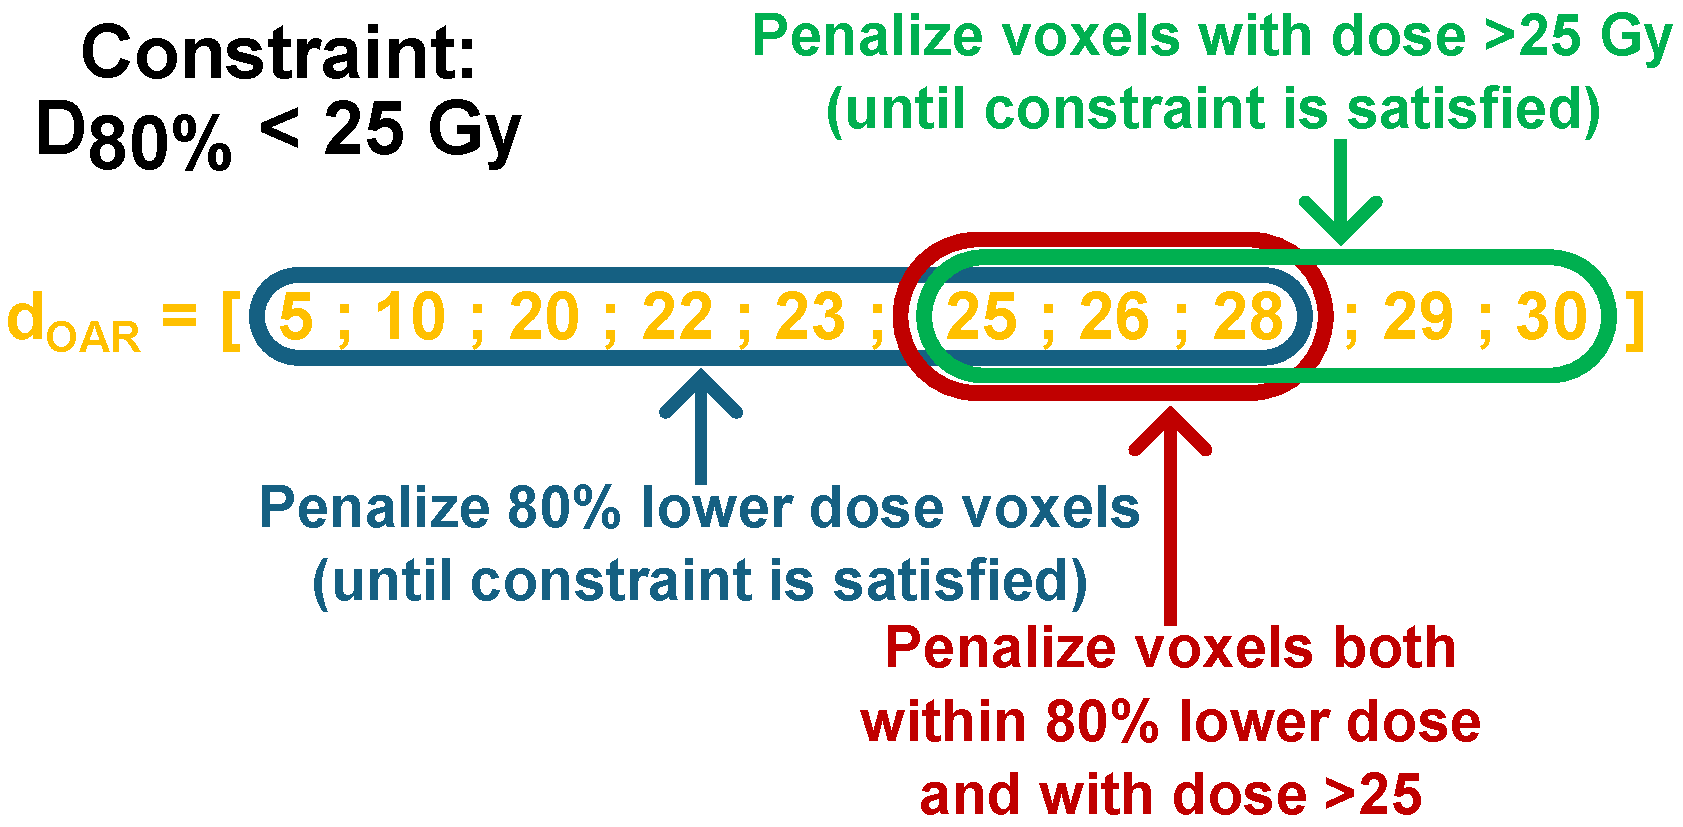
\includegraphics[width=0.6\textwidth]{constraint_penalization.pdf}
		\hfill
		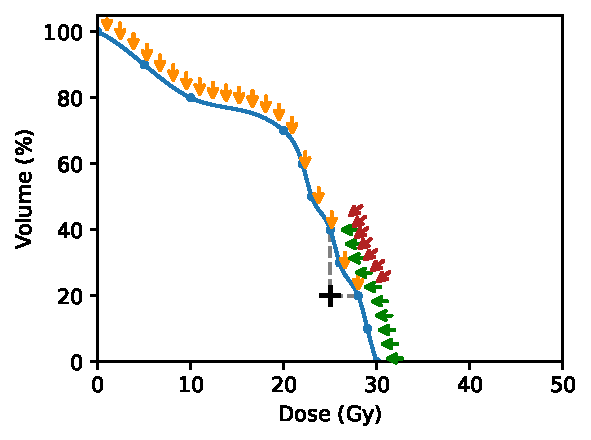
\includegraphics[width=0.35\textwidth]{constraint_penalization_plot.pdf}
		\caption{Penalizations of constraint $D_{20\%}< 25\,\text{Gy}$ on a structure of 10 voxels.}
		\label{fig:constraint_penalization_diagram}
	\end{subfigure}
	\\\vspace{3mm}
	\begin{subfigure}{0.32\textwidth}
		\centering
		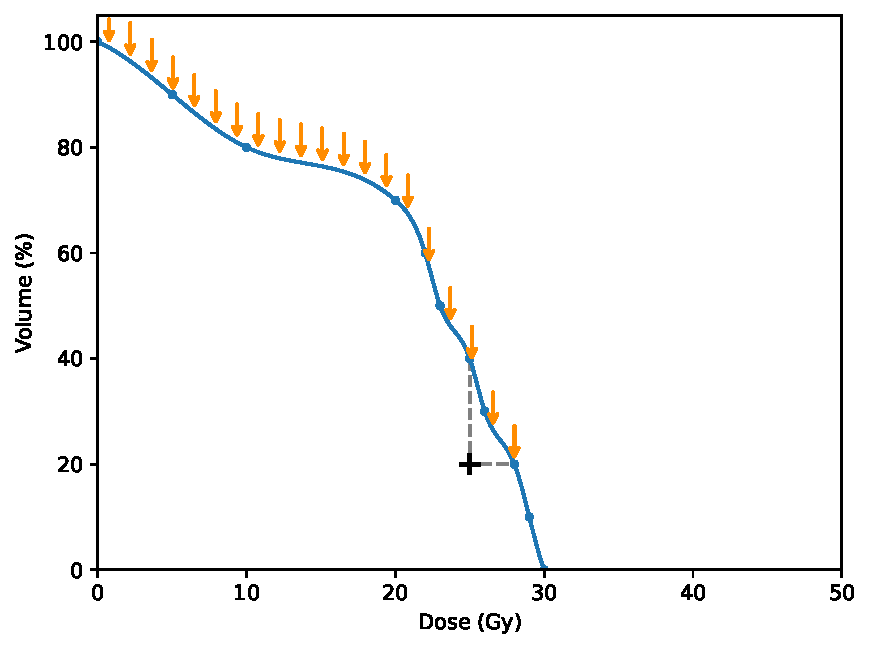
\includegraphics[width=0.9\textwidth]{constraint_penalization_plot_1.pdf}
		\caption{Penalizing the lower $20\,\%$ dose voxels.}
		\label{fig:constraint_penalization_plot_1}
	\end{subfigure}
	\begin{subfigure}{0.32\textwidth}
		\centering
		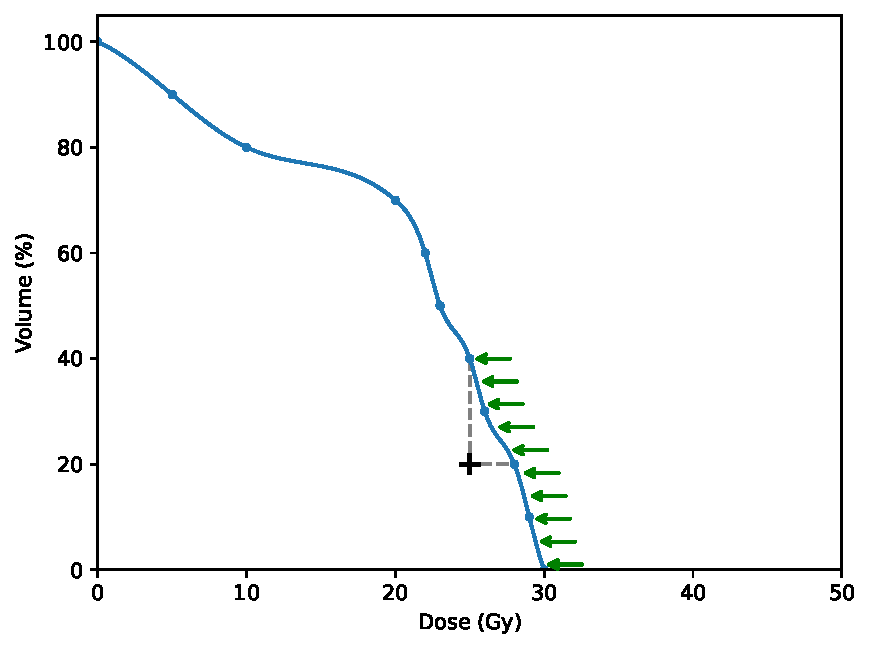
\includegraphics[width=0.9\textwidth]{constraint_penalization_plot_2.pdf}
		\caption{Penalizing voxels with dose greater than $25\,\text{Gy}$.}
		\label{fig:constraint_penalization_plot_2}
	\end{subfigure}
	\begin{subfigure}{0.32\textwidth}
		\centering
		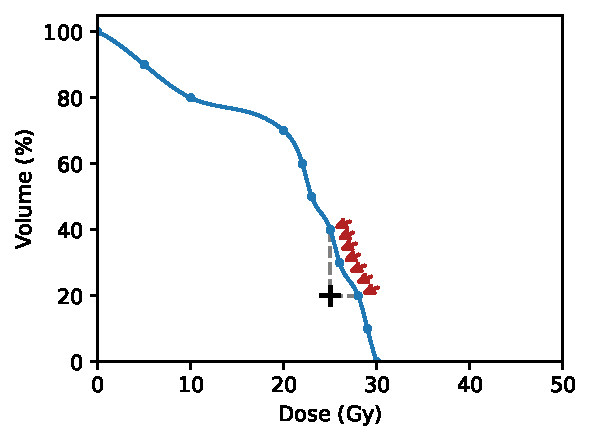
\includegraphics[width=0.9\textwidth]{constraint_penalization_plot_3.pdf}
		\caption{Penalizing the lower $20\,\%$ dose voxels with dose greater than $25\,\text{Gy}$.}
		\label{fig:constraint_penalization_plot_3}
	\end{subfigure}
	\caption{Typical penalization of a dose on an OAR according to the maximal dose constraint $D_{20\%} \leq 25\,\text{Gy}$.}
	\label{fig:constraint_penalization}
\end{figure}

Turning off penalization is possible once a constraint is met (this is useful for the first two methods presented above).
In our implementation, we chose not to do so, so when a constraint is on the edge of being met, the penalization does not turn on and off every other optimization iteration.

Once the set of penalized voxels is selected, the penalization power $p$ must be determined, with typical choices being $p=1$ or $p=2$.
We opt for penalizing voxels with a dose greater than $D$ Gy and set $p=2$.
This choice makes the objective function convex a weighted sum of convex functions.
Desirable properties, such as the existence of a unique global minimum once the values of $w_c$ are fixed, follow from the convexity of the objective function.

Finally, the mathematical formulation of the objective function associated with the constraint $c = \left( S, D, V, \pm \right)$ is:
$$f_c(\mathbf{d}) = \sum_{v \in S} \ReLU{\mathbf{d}_v - D}^2$$
and the global minimization problem becomes
$$
\min_{\mathbf{b}} \ \sum_{c \in \mathcal{C}} w_c \sum_{v \in S} \ReLU{\mathbf{d}_v - D}^2
\quad \text{ with }
\mathbf{d} = L\mathbf{b}, \ \mathbf{b} \geq 0
$$
where $w_c$, the weights or importance factors of each constraint, are to be determined.

\subsection{Balancing the Importance Factors}
The importance factors $w_c$ play a crucial role in the optimization process.
These weights allow dosimetrists to prioritize certain clinical constraints over others.
Properly balancing these factors ensures that the most critical aspects of the treatment plan are emphasized while still striving to meet all constraints.

The constraints associated with the PTV, ensuring the destruction of the tumor, conflict with the protection of the OARs.
Hence, the optimization process becomes a trade-off between satisfying different constraints.
For example, increasing the dose of the PTV will inadvertently increase the dose of nearby OARs.
Carefully tuning of the importance factors ensures that the optimization algorithm directs the fluence maps towards a solution that balances the therapeutic benefits with the risk of complications.

Due to the unique geometry of each patient, an optimal dose plan cannot be applied universally.
The optimization must be recalculated for every patient.
Dosimetrists customize the dose to meet the specific needs of each individual patient by taking into account clinical priorities, spatial relationships, and physician expertise.
This process is time consuming, and remains manual; this manuscript tackles the problem of treatment planning.

The contouring task used to be a manual operation but is now done automatically, thanks to the progress of artificial intelligence on segmentation tasks \cite{Kim2024} \cite{Duan2022}.
After the emergence of AI for contouring, this manuscript tackles the problem of automatic treatment planning.

\section{Dose Mimicking}
Dose mimicking is a technique used to reproduce a dose distribution as closely as possible.
It involves the optimization of a new treatment plan to match the dose profile of an existing plan, which is typically derived from either a prior treatment or a reference plan considered clinically acceptable.
This differ from the naive approach in \ref{naive_optimization}: the dose distribution that we try to replicate is not manually set.
The target dose was achieved before either on the same machine, or on a similar MLC.
Hence, the task of mimicking it should be "easier".

Formally, the optimization problem can be stated the same way as in \ref{naive_optimization}:
$$ \min_\mathbf{b} \ \| \mathbf{d}_{\text{target}} - L\mathbf{b} \|^2 $$
with $\mathbf{d}_{\text{target}}$ the previously target dose, instead of the manually defined one.

\section{Optimization Algorithm Review for Dosimetry}
The selection of an optimization algorithm is critical.
Different algorithms may converge to various local minima when dealing with non-convex objective functions, potentially leading to significant outcome variations.
To mitigate this issue, we have designed the objective function to be convex, ensuring all optimization methods converge to the same global minimum.
In this study, we benchmark the computational complexity and convergence rates of various algorithms.
These findings are intended to provide valuable insights for the development of TPS.
% This was published as an ArXiV paper

\subsection{Data}
We focused on evaluating the various open-source optimizers.
We used the widely recognized TG-119 \cite{AAPM-TG119} cases as a benchmark for evaluating radiation therapy plan optimization.
The TG-119 dataset provides specific dose goals, which we incorporated into our proposed cost function.
The TGG 119 multiple PTVs is a theoretical case unlikely to happen in real life.
However, the other cases represent a comprehensive set of what dosimetrists could encounter daily.

We also used one typical case of prostate cancer from ICM.
For this case, doctors had provided specific dose goals that we again incorporated into our proposed cost function.

\subsection{Open-source Optimizers}
We tried to have a comprehensive set of available open-source optimizers.
\paragraph{(Stochastic) Gradient Descent}
Is an optimization algorithm that iteratively updates the model parameters in the direction of the negative gradient of the objective function.
In our case, it is not stochastic since it calculates the gradient using the current solution\footnote{Our objective function has all its inputs as parameters, so there is no notion of stochasticity.} \cite{Lemarechal2012}.
\paragraph{Conjugate Gradient}
Is an iterative optimization algorithm commonly used to solve systems of linear equations or quadratic optimization problems.
It iteratively computes conjugate directions and updates the solution along them, aiming to minimize the objective function \cite{Hestenes1952}.
Conjugate Gradient is often applied in scenarios where the Hessian matrix is unavailable or computationally expensive.
\paragraph{Newton}
Newton's method is an iterative optimization algorithm that uses the second-order derivative (Hessian matrix) to find the minimum of a function.
It updates the current estimate by considering both the first-order derivative (gradient) and the second-order derivative \cite{Nocedal06}.
\paragraph{SLSQP}
(Sequential Least Squares Programming) is a sequential quadratic programming algorithm for constrained optimization.
It iteratively solves a sequence of quadratic programming subproblems to find the optimal solution subject to constraints \cite{Bonnans2006}.
\paragraph{RMSprop}
(Root Mean Square Propagation) is an optimization algorithm that addresses the problem of diminishing learning rates in traditional gradient descent methods.
It divides the learning rate by the root mean square of the past gradients, which helps to stabilize and speed up convergence \cite{Hinton2012}.
\paragraph{BFGS-based}
\subparagraph{Pure BFGS}
(Broyden-Fletcher-Goldfarb-Shanno) is a quasi-Newton method that approximates the Hessian matrix using updates based on gradient information.
It performs a line search to determine the step size that minimizes the objective function along the search direction \cite{Fletcher1987}.
\subparagraph{L-BFGS}
(Limited-memory BFGS) is a variation of BFGS that uses a limited-memory approach to approximate the Hessian matrix.
It stores a limited number of past gradient and parameter values to compute an approximate inverse Hessian matrix efficiently \cite{Liu1989}.
\paragraph{Adam-based}
\subparagraph{Pure Adam}
(Adaptive Moment Estimation) is an optimization algorithm combining ideas from adaptive learning rates and momentum methods.
It computes adaptive learning rates for each parameter based on estimates of the first and second moments of the gradients \cite{Kingma2017}.
\subparagraph{RAdam}
(Rectified Adam) is a variant of the Adam optimizer that introduces a rectification term to stabilize the adaptive learning rate.
It aims to address some convergence issues that may occur in Adam by dynamically adjusting the variance of the adaptive learning rate \cite{Liu2021}.
\subparagraph{NAdam}
(Nesterov Adam) combines the Nesterov accelerated gradient method with the Adam optimizer.
It incorporates Nesterov momentum into the Adam update rule to improve convergence and provide better generalization \cite{Tato2018}.
\subparagraph{AdamDelta}
Is another variant of the Adam optimizer that replaces the second moment estimates (variance) with a delta parameter.
It eliminates the need for storing and updating the moving average of the squared gradients, which can be beneficial in memory-constrained settings \cite{Zeiler2012}.
\subparagraph{Adamax}
Is an extension of the Adam optimizer that uses the gradients' infinity norm (max norm) instead of the L2 norm. It is designed to handle sparse gradients more effectively and can be particularly useful in deep learning models \cite{Bera2020}.
\paragraph{Rprop}
(Resilient Backpropagation) is an optimization algorithm specifically designed for neural networks.
It adaptively updates the weights based on the gradient sign, adjusting the step size.
Rprop performs weight updates independently for each weight parameter \cite{Riedmiller1992}.
\paragraph{Other optimizers variations}
In addition, we tested AdamW, Adagrad, and ASGD.
However, AdamW and Adagrad behaved similarly to Adam, and ASGD behaved similarly to SGD.
For readability purposes, we did not include them in the results plots.

\subsection{Results}

\begin{figure}
	\centering
	\begin{subfigure}{\textwidth}
		\centering
		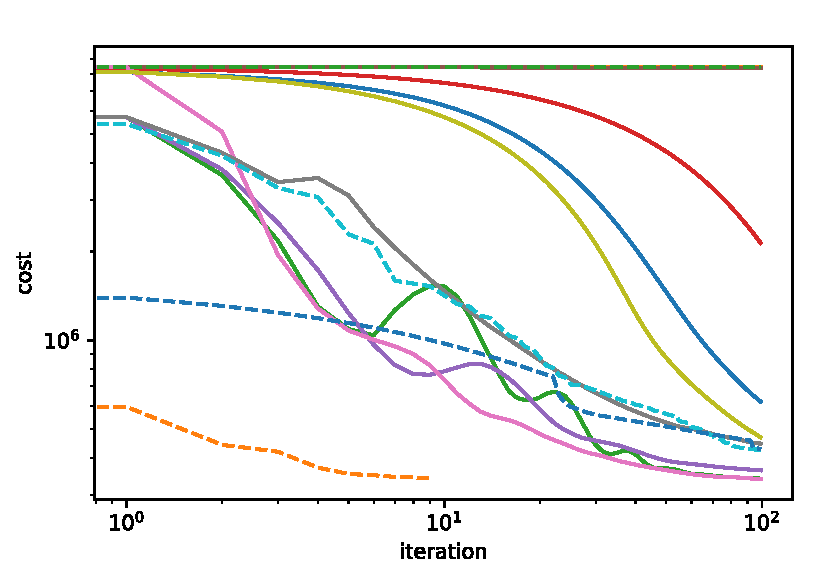
\includegraphics[height=5cm]{optimizers_comparison/TGG119Multi-iter.pdf}
		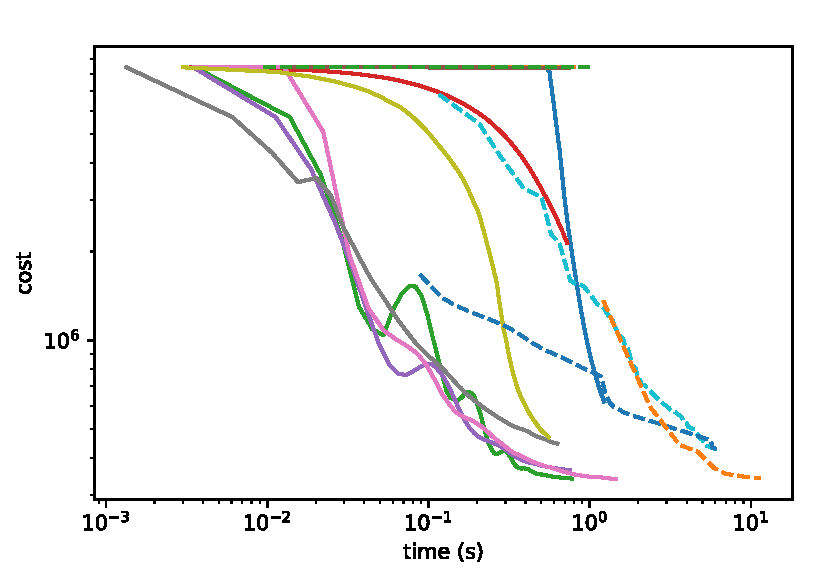
\includegraphics[height=5cm]{optimizers_comparison/TGG119Multi-time.pdf}
		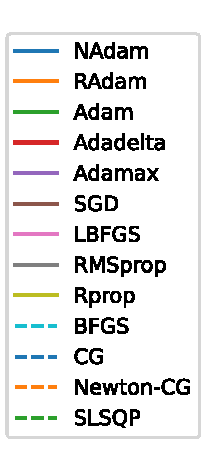
\includegraphics[height=5cm]{optimizers_comparison/legend.pdf}
		\caption{TGG 119: Multiple PTVs.}
		\label{fig:TGG119_Multi}
	\end{subfigure}
	\begin{subfigure}{\textwidth}
		\centering
		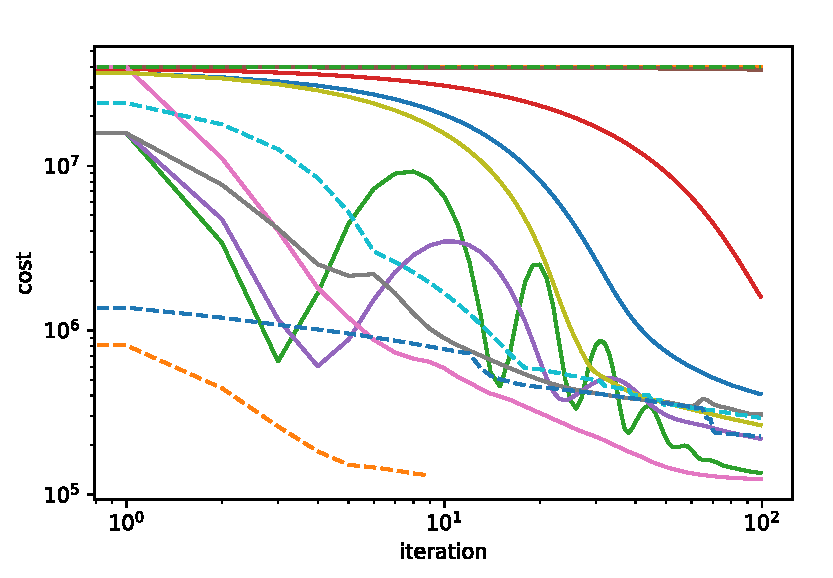
\includegraphics[height=5cm]{optimizers_comparison/TGG119HN-iter.pdf}
		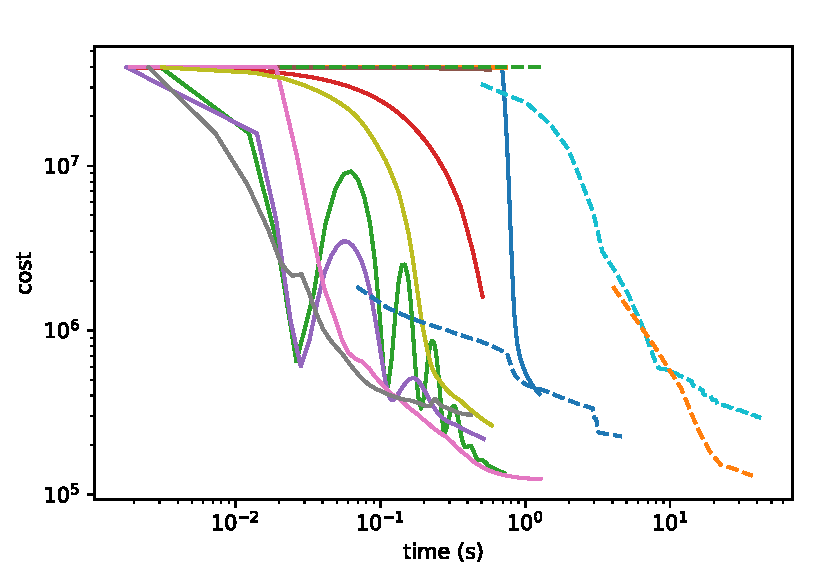
\includegraphics[height=5cm]{optimizers_comparison/TGG119HN-time.pdf}
		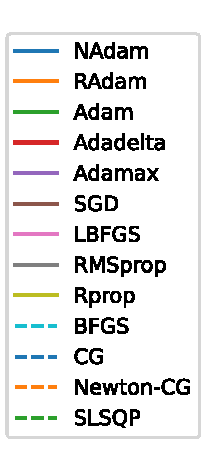
\includegraphics[height=5cm]{optimizers_comparison/legend.pdf}
		\caption{TGG 119: Head and Neck.}
		\label{fig:TGG119_HN}
	\end{subfigure}
	\begin{subfigure}{\textwidth}
		\centering
		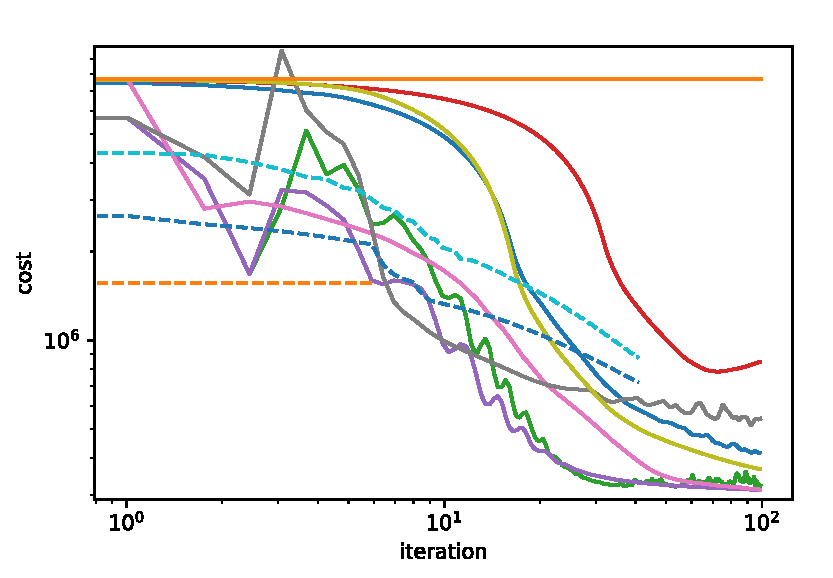
\includegraphics[height=5cm]{optimizers_comparison/TGG119Prostate-iter.pdf}
		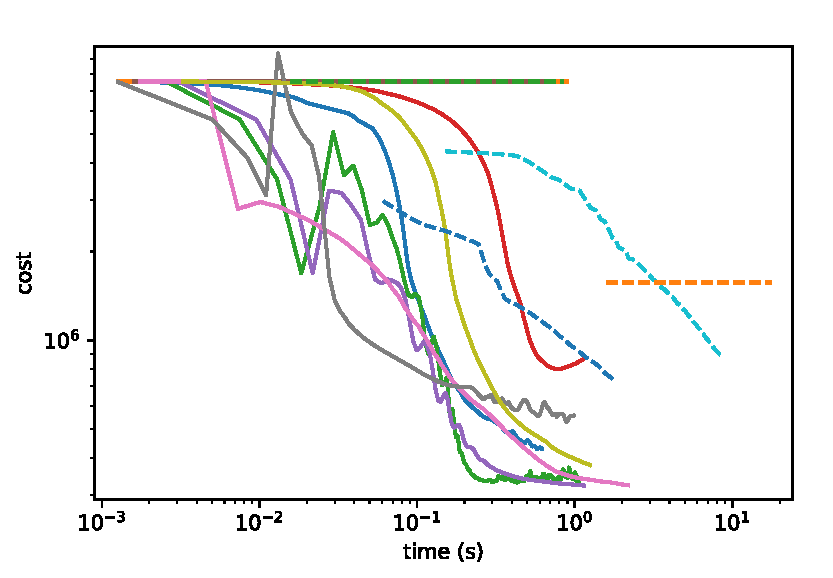
\includegraphics[height=5cm]{optimizers_comparison/TGG119Prostate-time.pdf}
		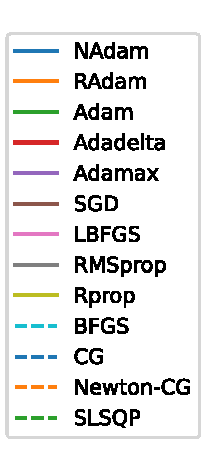
\includegraphics[height=5cm]{optimizers_comparison/legend.pdf}
		\caption{TGG 119: Prostate.}
		\label{fig:TGG119_Prostate}
	\end{subfigure}
	\begin{subfigure}{\textwidth}
		\centering
		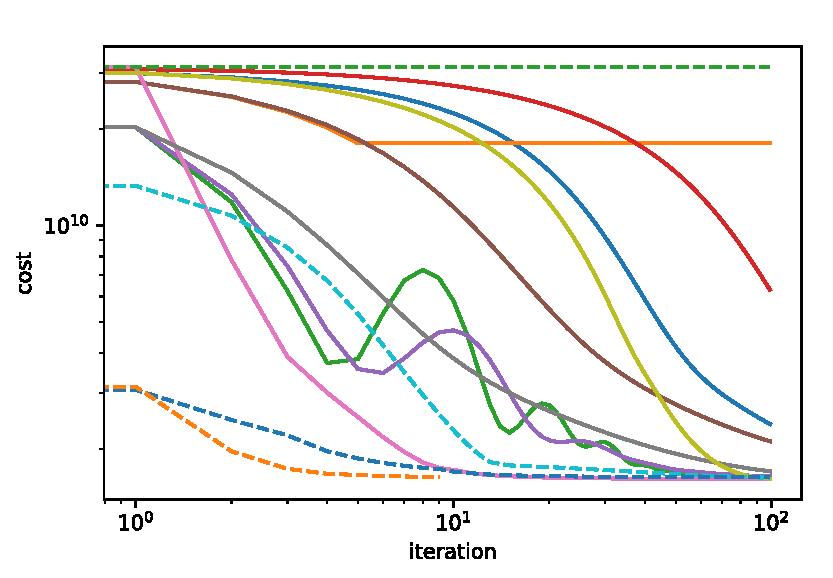
\includegraphics[height=5cm]{optimizers_comparison/ICMProstate-iter.pdf}
		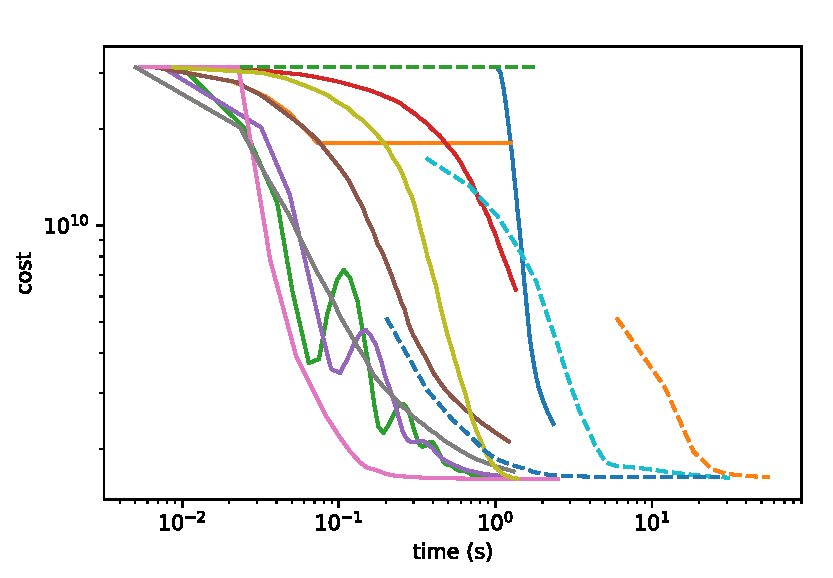
\includegraphics[height=5cm]{optimizers_comparison/ICMProstate-time.pdf}
		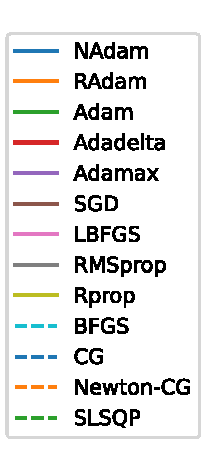
\includegraphics[height=5cm]{optimizers_comparison/legend.pdf}
		\caption{Prostate from ICM (Institut régonal du Cancer de Montpellier).}
		\label{fig:ICM_Prostate}
	\end{subfigure}
	\caption{Evolution of the objective function value ('cost') through optimization iterations and computation time for four typical dosimetry cases.}
	\label{fig:OptimizersComparison}
\end{figure}

\paragraph{Newton's method}
Based on the iterations-wise graph analysis, Newton's method performs best, consistently achieving a stable converged state within ten steps across all four examined cases.
However, Newton's method steps are computationally expensive since it uses a second-order derivative (the Hessian) that is difficult to compute.

It is widely recognized that Newton's method excels in optimizing convex functions \cite{PoczosTibshirani2013}.
Our objective function is convex by construction; hence, this optimization algorithm is particularly effective.

\paragraph{LBFGS vs BFGS}
It would be expected that BFGS performs better than LBFGS in terms of iterations but not in terms of time (since LBFGS is a fast approximation of the BFGS technique).
However, we observe that LBFGS outperforms BFGS even on the iterations-wise graph.
This performance suggests that the limited memory approximation is biased towards suitable directions in these problems.

\paragraph{Best Algorithms}
Besides Newton's method, three algorithms have similar performances: Adam, Adamax, and LBFGS.
Adam and Adamax appear to have more "wavy" cost curves, while LBFGS cost decreases more stably.
These observations are valid both in terms of iteration and time.

TGG 119 Multiple PTVs (figure \ref{fig:TGG119_Multi}) is the smallest problem, and the real ICM prostate case (figure \ref{fig:ICM_Prostate}) is the largest problem (in terms of patient/organs/structure volume size);
TGG 119 fake head and neck (figure \ref{fig:TGG119_HN}) and TGG 119 fake prostate (figure \ref{fig:TGG119_Prostate}) have similar sizes.
Notably, an observable trend indicates that as the problem size increases, LBFGS outperforms both Adamax and Adam optimization algorithms.

Therefore, we will use the LBFGS algorithm in the rest of this manuscript.

\subsection{Discussion}
In the future, if new techniques are developed one day, making computing the Hessian much faster, we recommend using Newton's optimization algorithm.
However, to our knowledge, computing the Hessian remains long, not only in our implementation.

Hence, we recommend using the LBFGS algorithm for the problem of dose optimization in radiotherapy;
it is the fastest to converge and converges steadily on the tested cases.
